\documentclass[11pt,a4paper]{article}

% Image mode: pdf.
% Image paths stay relative. In PDF mode, place same-basename PDF conversions
% of the chapter SVG files in the assets/ directory beside this source.

\usepackage{iftex}
\ifPDFTeX
  \PackageError{handout}{This template requires XeTeX or Tectonic}{Compile with xelatex or tectonic.}
\fi

\usepackage[a4paper,top=18mm,bottom=20mm,left=20mm,right=20mm,headsep=6mm]{geometry}
\usepackage{fontspec}
\usepackage{xeCJK}
\usepackage{amsmath}
\usepackage{unicode-math}

% Font settings are intentionally visible in the generated .tex file.
% These defaults target the macOS machine used for the released PDF.
% Change the family names when compiling on another system.
\setmainfont{Songti TC}
\setsansfont{Heiti TC}
\setmonofont{Menlo}
\setCJKmainfont{Songti TC}
\setCJKsansfont{Heiti TC}
\setCJKmonofont{Heiti TC}
\setmathfont{STIX Two Math}
\XeTeXlinebreaklocale "zh"
\XeTeXlinebreakskip=0pt plus 1pt

\usepackage{xcolor}
\definecolor{HandoutBlue}{HTML}{215A91}
\definecolor{HandoutBlueLight}{HTML}{EEF5FC}
\definecolor{HandoutGreen}{HTML}{39715A}
\definecolor{HandoutGreenLight}{HTML}{EFF8F3}
\definecolor{HandoutGold}{HTML}{8A641C}
\definecolor{HandoutGoldLight}{HTML}{FFF8E8}
\definecolor{HandoutInk}{HTML}{253142}
\definecolor{HandoutMuted}{HTML}{667085}

\usepackage{graphicx}
\makeatletter
% Pandoc 3 emits an accessibility `alt` key for raster/PDF images. Older
% graphicx releases do not know that key, so accept it without changing layout.
\@ifundefined{KV@Gin@alt}{\define@key{Gin}{alt}{}}{}
\newsavebox\pandoc@box
\newcommand*\pandocbounded[1]{%
  \sbox\pandoc@box{#1}%
  \Gscale@div\@tempa{\textheight}{\dimexpr\ht\pandoc@box+\dp\pandoc@box\relax}%
  \Gscale@div\@tempb{\linewidth}{\wd\pandoc@box}%
  \ifdim\@tempb\p@<\@tempa\p@\let\@tempa\@tempb\fi
  \ifdim\@tempa\p@<\p@\scalebox{\@tempa}{\usebox\pandoc@box}%
  \else\usebox{\pandoc@box}%
  \fi
}
\makeatother
\usepackage{float}
\floatplacement{figure}{H}
% Pandoc uses LTcaptype=none for uncaptioned longtables. The caption package
% expects that name to exist as a counter even though it is never displayed.
\newcounter{none}
\usepackage{caption}
\captionsetup[figure]{labelformat=empty,labelsep=none,font=small}

\usepackage{booktabs,longtable,array,calc}
\usepackage{etoolbox}
\makeatletter
\patchcmd\longtable{\par}{\if@noskipsec\mbox{}\fi\par}{}{}
\makeatother

\usepackage[most]{tcolorbox}
\tcbuselibrary{breakable,skins}
\newtcolorbox{HandoutLearningMap}{
  enhanced,breakable,colback=HandoutBlueLight,colframe=HandoutBlue,
  boxrule=0.8pt,arc=1.5mm,left=3mm,right=3mm,top=2mm,bottom=2mm,
  before skip=8pt,after skip=10pt
}
\newtcolorbox{HandoutWorkedExample}{
  enhanced,breakable,colback=HandoutGreenLight,colframe=HandoutGreen,
  boxrule=0.65pt,arc=1.5mm,left=3mm,right=3mm,top=2mm,bottom=2mm,
  before skip=8pt,after skip=10pt
}
\newtcolorbox{HandoutSelfCheck}{
  enhanced,breakable,colback=HandoutGoldLight,colframe=HandoutGold,
  boxrule=0.65pt,arc=1.5mm,left=3mm,right=3mm,top=2mm,bottom=2mm,
  before skip=8pt,after skip=10pt
}

\usepackage{titlesec}
\titleformat{\section}{\sffamily\bfseries\Large\color{HandoutBlue}}{}{0pt}{}
\titleformat{\subsection}{\sffamily\bfseries\large\color{HandoutInk}}{}{0pt}{}
\titleformat{\subsubsection}{\sffamily\bfseries\normalsize\color{HandoutInk}}{}{0pt}{}
\titlespacing*{\section}{0pt}{1.4em}{0.55em}
\titlespacing*{\subsection}{0pt}{1.15em}{0.45em}
\titlespacing*{\subsubsection}{0pt}{0.9em}{0.35em}
\setcounter{secnumdepth}{-\maxdimen}

\usepackage{hyperref}
\usepackage{bookmark}
\IfFileExists{xurl.sty}{\usepackage{xurl}}{}
\urlstyle{same}
\hypersetup{
  colorlinks=true,
  linkcolor=HandoutBlue,
  urlcolor=HandoutBlue,
  citecolor=HandoutBlue,
  pdftitle={必物-4 電與磁的統一},
  pdfsubject={物理},
  pdfcreator={Pandoc with the HighSchooContent LaTeX template}
}

\setlength{\parindent}{0pt}
\setlength{\parskip}{0.55em plus 0.15em minus 0.1em}
\setlength{\emergencystretch}{3em}
\setlength{\LTpre}{0.5em}
\setlength{\LTpost}{0.5em}
\renewcommand{\arraystretch}{1.18}
\providecommand{\tightlist}{%
  \setlength{\itemsep}{0pt}\setlength{\parskip}{0pt}}
\pagestyle{plain}


\begin{document}

\begin{tcolorbox}[
  enhanced,colback=white,colframe=HandoutBlue,boxrule=1.1pt,arc=2mm,
  borderline west={3pt}{0pt}{HandoutBlue},left=5mm,right=4mm,top=4mm,bottom=4mm
]
{\sffamily\small\bfseries\color{HandoutBlue}學生講義}\par
{\sffamily\bfseries\LARGE\color{HandoutInk}必物-4 電與磁的統一}\par
\vspace{0.35em}{\large 從電流與磁場、波前與光路，建立發電、通訊、光學與測速的共同模型}\par
\vspace{0.45em}{\small\color{HandoutMuted}%
科目：物理
\quad 課程：普通高中必修物理
\quad 版本：學生版｜核心＋理解
\quad 校訂：2026-08-29
}\par
\vspace{0.25em}{\small\color{HandoutMuted}範圍：現行必修主線；含電流磁效應、電磁感應、電磁波、光波與都卜勒效應}\par
\end{tcolorbox}


電能可以轉成馬達的轉動，轉動也可以在發電機中轉成電能；天線中的振盪電流能把訊號送到遠方，光也能用同一套波動模型分析反射、折射、干涉與繞射。本章把這些現象接成一條因果鏈：\textbf{電流建立磁場，變動的磁場建立電場，變動的電場與磁場能在空間中傳播。}

這套模型直接參與發電、變壓、感應充電、家用電路保護、無線通訊、光纖、光譜分析、超音波與雷達測速。

\begin{HandoutLearningMap}

\subsection{本章核心關係}\label{ux672cux7ae0ux6838ux5fc3ux95dcux4fc2}

\begin{enumerate}
\def\labelenumi{\arabic{enumi}.}
\tightlist
\item
  \textbf{電流與磁場}：電流周圍有磁場；方向由電流方向與幾何形狀共同決定。
\item
  \textbf{磁場與受力}：外加磁場對載流導線施力，線圈兩側的磁力形成轉動效果。
\item
  \textbf{電磁感應}：穿過線圈的磁通量改變時，線圈中出現感應電動勢；感應磁場抵抗原來的磁通量變化。
\item
  \textbf{能量轉換與安全}：發電機、變壓器、感應爐與無線充電都利用電磁感應；家庭各支路並聯，保險絲、無熔絲開關、接地與漏電斷路器分別處理不同風險。
\item
  \textbf{電磁波}：互相變動的電場與磁場可離開電荷與電流，在空間中傳遞能量。
\item
  \textbf{週期波}：振幅、週期、頻率、波長與波速描述波；同一波源在固定介質中滿足 \(v=f\lambda\)。
\item
  \textbf{光的波動}：波前模型導出反射與折射，疊加原理解釋干涉，有限孔徑造成繞射。
\item
  \textbf{都卜勒效應}：波源或觀察者沿視線相對運動時，接收到的頻率改變；測得的是徑向運動資訊。
\end{enumerate}

\end{HandoutLearningMap}

\section{1. 電流建立磁場，磁場也能推動電流}\label{ux96fbux6d41ux5efaux7acbux78c1ux5834ux78c1ux5834ux4e5fux80fdux63a8ux52d5ux96fbux6d41}

\subsection{1.1 電流的磁效應}\label{ux96fbux6d41ux7684ux78c1ux6548ux61c9}

厄斯特把通電導線放在指南針附近，觀察到磁針轉向；切斷電流後，磁針回到原來方向。反轉電流，磁針偏轉方向也反轉。這組對照把因果關係鎖定在電流：\textbf{移動的電荷會建立磁場。}

圖 1 先固定電流方向，再由右手定則讀出各位置的磁場方向。圓點 \(\odot\) 表示向紙面外，叉號 \(\otimes\) 表示向紙面內。

\begin{figure}
\centering
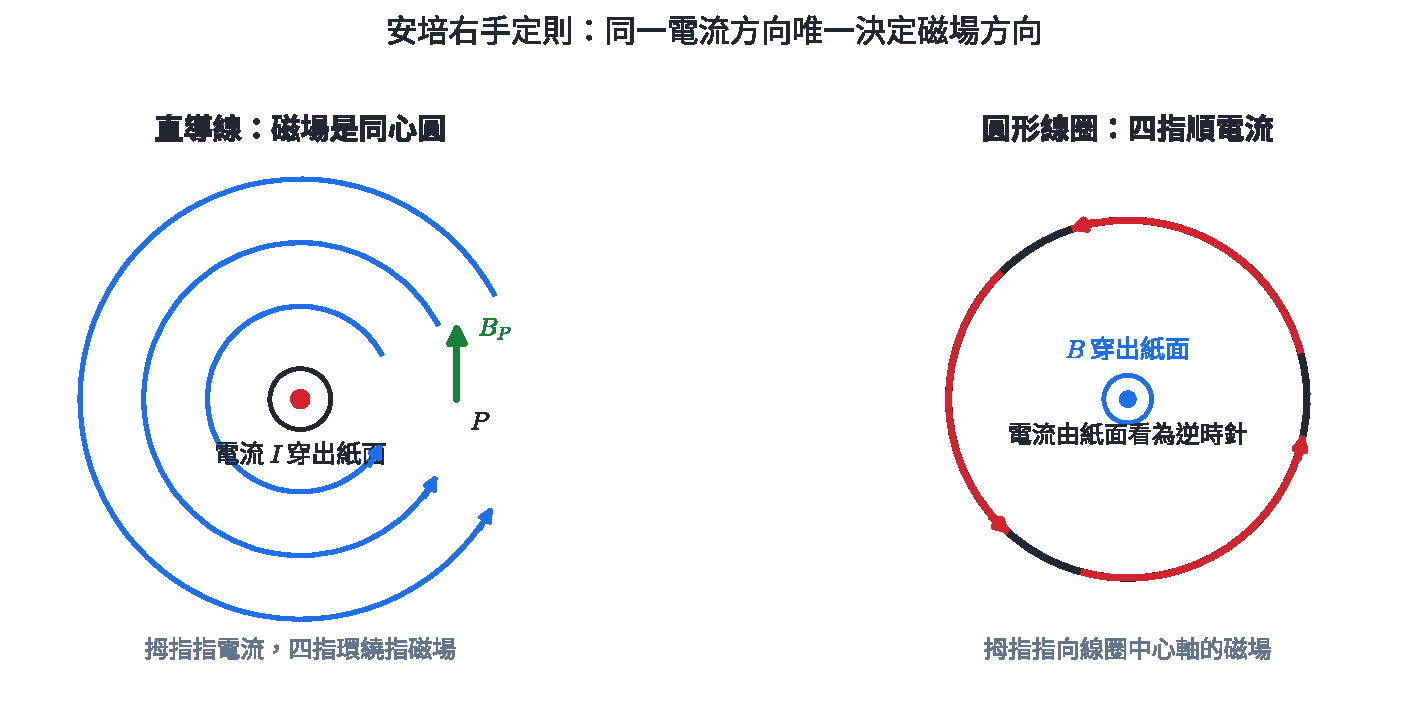
\includegraphics[width=0.96\linewidth,height=\textheight,keepaspectratio,alt={圖 1｜直導線的磁場沿同心圓切線；圓形線圈中心的磁場沿線圈軸。}]{assets/必物-4-直導線與線圈磁場.pdf}
\caption{圖 1｜直導線的磁場沿同心圓切線；圓形線圈中心的磁場沿線圈軸。}
\end{figure}

\subsubsection{直導線}\label{ux76f4ux5c0eux7dda}

右手拇指指向\textbf{傳統電流}，彎曲四指的環繞方向就是磁場方向。直導線周圍每一點的磁場都沿以導線為圓心的圓周切線。

在相同介質中，量值的核心比例為

\[
B_{\text{直導線}}\propto\frac{I}{r}.
\]

電流 \(I\) 越大，磁場越強；距離 \(r\) 越遠，磁場越弱。電子在金屬中的漂移方向與傳統電流方向相反，右手定則使用傳統電流。

\subsubsection{圓形線圈與螺線管}\label{ux5713ux5f62ux7ddaux5708ux8207ux87baux7ddaux7ba1}

四指沿線圈的傳統電流方向彎曲，拇指指出線圈中心軸的磁場方向。增加匝數會讓各匝磁場同向疊加：

\[
B_{\text{圓形線圈中心}}\propto\frac{NI}{R},
\qquad
B_{\text{長螺線管內}}\propto nI.
\]

\(N\) 是總匝數，\(R\) 是線圈半徑，\(n\) 是單位長度匝數。鐵芯容易被磁化，把磁場集中在螺線管內，因此電磁鐵、繼電器與電磁門鎖常在線圈中加入鐵芯。

多條導線同時存在時，每條導線各自建立磁場，總磁場由向量疊加：

\[
\vec B_{\text{合}}=\vec B_1+\vec B_2+\cdots.
\]

\begin{HandoutWorkedExample}

\subsection{完整示範 1｜兩條直導線在中點的磁場}\label{ux5b8cux6574ux793aux7bc4-1ux5169ux689dux76f4ux5c0eux7ddaux5728ux4e2dux9edeux7684ux78c1ux5834}

兩條長直導線垂直紙面，分別位於 \(x=-a\) 與 \(x=+a\)。左導線電流穿出紙面，右導線電流穿入紙面，兩電流量值相同。求原點的合磁場方向。

\textbf{先畫每條導線在原點的半徑方向：}

\begin{itemize}
\tightlist
\item
  原點位於左導線右側。左導線電流穿出紙面，磁場逆時針，因此原點處磁場向上。
\item
  原點位於右導線左側。右導線電流穿入紙面，磁場順時針，因此原點處磁場也向上。
\end{itemize}

兩個磁場同向且量值相同，合磁場向上，量值是單一導線在該處磁場的 2 倍。

\textbf{檢查：}把兩電流同時反向，兩個磁場都轉為向下，合磁場也反向。

\end{HandoutWorkedExample}

\begin{HandoutWorkedExample}

\subsection{完整示範 2｜用指南針檢驗磁場強弱}\label{ux5b8cux6574ux793aux7bc4-2ux7528ux6307ux5357ux91ddux6aa2ux9a57ux78c1ux5834ux5f37ux5f31}

一條南北向直導線放在指南針上方。第一次通入 \(0.50\ \mathrm A\)，第二次通入 \(1.00\ \mathrm A\)，導線與磁針距離不變。比較兩次導線磁場與磁針偏轉。

由 \(B\propto I/r\)，第二次電流是 2 倍，因此導線在磁針處建立的磁場是 2 倍。磁針同時受地磁場與導線磁場影響，平衡方向沿兩者的向量合成；導線磁場增加後，磁針會更偏向導線磁場方向。

實驗採低電壓電源並限制通電時間，避免導線因大電流過熱。若要公平比較電流效應，導線位置、指南針位置與周圍鐵磁物體都要固定。

\end{HandoutWorkedExample}

\subsection{1.2 外加磁場對載流導線施力}\label{ux5916ux52a0ux78c1ux5834ux5c0dux8f09ux6d41ux5c0eux7ddaux65bdux529b}

磁場中的移動電荷受到磁力；在一段導線中，許多載流子的磁力合成為導線所受的力。圖 2 先給出磁場、電流與兩側受力，兩力形成一對轉動效果。

\begin{figure}
\centering
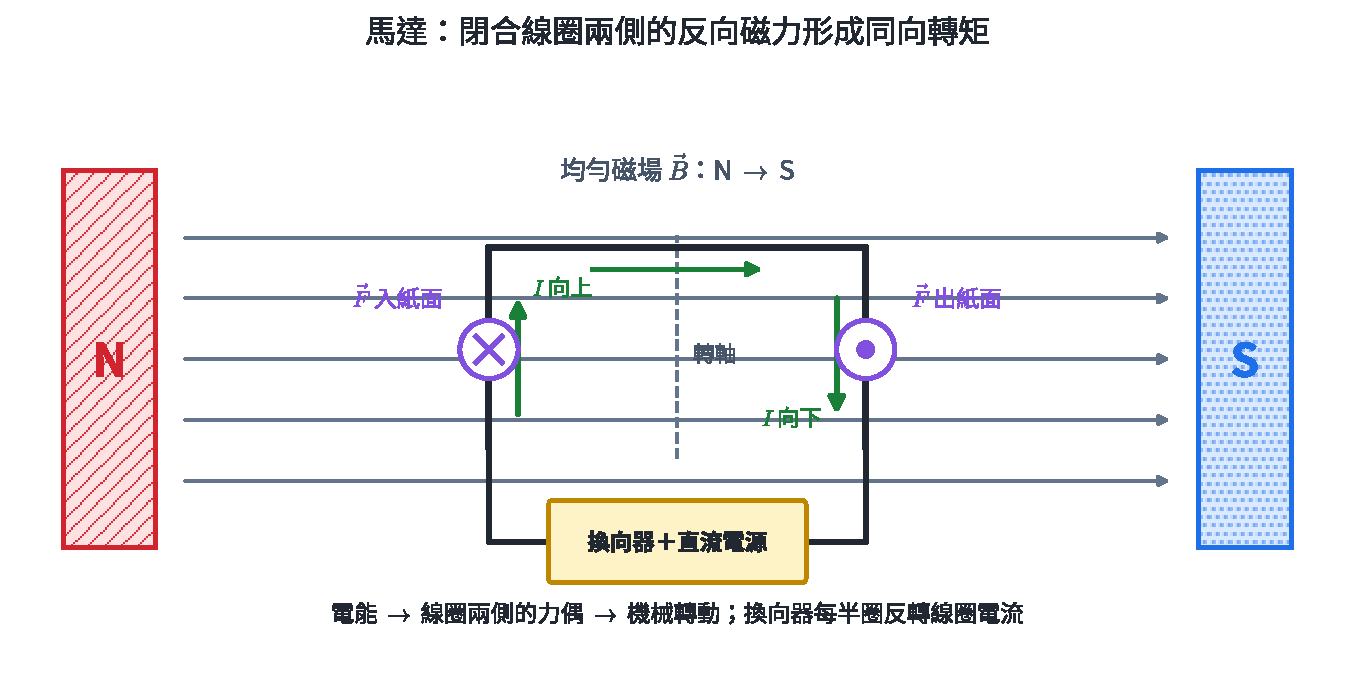
\includegraphics[width=0.94\linewidth,height=\textheight,keepaspectratio,alt={圖 2｜磁場由 N 指向 S；閉合線圈左側電流向上、磁力入紙面，右側電流向下、磁力出紙面，兩力對轉軸產生同向轉矩。}]{assets/必物-4-馬達線圈受力.pdf}
\caption{圖 2｜磁場由 N 指向 S；閉合線圈左側電流向上、磁力入紙面，右側電流向下、磁力出紙面，兩力對轉軸產生同向轉矩。}
\end{figure}

長度為 \(L\) 的直導線通以電流 \(I\)，放在均勻磁場 \(B\) 中；導線方向與磁場夾角為 \(\theta\) 時，

\[
F=ILB\sin\theta.
\]

方向可由

\[
\vec F=I\vec L\times\vec B
\]

判定：右手四指由電流方向轉向磁場方向，拇指指向磁力。由公式可直接讀出三個條件：

\begin{itemize}
\tightlist
\item
  導線與磁場垂直時，\(\sin90^\circ=1\)，磁力最大。
\item
  導線與磁場平行時，\(\sin0^\circ=0\)，磁力為零。
\item
  反轉電流或反轉磁場其中一項，磁力反向；兩者同時反轉，磁力維持原方向。
\end{itemize}

馬達把線圈放在磁場中，讓線圈相對兩側受到方向相反的力而轉動。線圈轉過半圈後，換向器改變線圈電流方向，使轉矩持續朝同一轉向。揚聲器則讓音訊交流電通過音圈；電流隨時間改變，磁力帶動振膜往復，形成聲波。

\begin{HandoutWorkedExample}

\subsection{完整示範 3｜載流導線的受力大小與方向}\label{ux5b8cux6574ux793aux7bc4-3ux8f09ux6d41ux5c0eux7ddaux7684ux53d7ux529bux5927ux5c0fux8207ux65b9ux5411}

長 \(0.20\ \mathrm m\) 的直導線通以 \(3.0\ \mathrm A\) 電流，垂直放在 \(0.50\ \mathrm T\) 的均勻磁場中。磁場向右，電流穿出紙面。求磁力。

\textbf{大小：}

\[
F=ILB\sin90^\circ
=(3.0)(0.20)(0.50)=0.30\ \mathrm N.
\]

\textbf{方向：}電流為 \(+z\)，磁場為 \(+x\)，所以

\[
(+z)\times(+x)=+y.
\]

磁力向上。

\textbf{檢查：}若導線旋轉到與磁場夾 \(30^\circ\)，力會變成 \(0.30\sin30^\circ=0.15\ \mathrm N\)；方向仍垂直於電流與磁場共同張成的平面。

\end{HandoutWorkedExample}

\begin{HandoutSelfCheck}

\subsection{本節獨立練習}\label{ux672cux7bc0ux7368ux7acbux7df4ux7fd2}

\begin{enumerate}
\def\labelenumi{\arabic{enumi}.}
\tightlist
\item
  一條直導線的電流穿入紙面。導線正上方一點的磁場指向哪裡？
\item
  圓形線圈由紙面正面看，電流為順時針。線圈中心磁場朝紙面內或外？
\item
  長螺線管的長度與電流固定，總匝數變為原來 \(1.5\) 倍。管內磁場近似變為幾倍？
\item
  兩條平行直導線電流同向。用其中一條導線建立的磁場判斷另一條導線所受磁力，兩線互相吸引或排斥？
\item
  揚聲器輸入的交流電反轉方向時，音圈的磁力如何改變？這項改變如何形成聲波？
\end{enumerate}

\textbf{簡答：}1. 向右。2. 朝紙面內。3. \(1.5\) 倍。4. 互相吸引。5. 磁力反向，音圈與振膜往復振動並推動空氣。

\end{HandoutSelfCheck}

\section{2. 磁通量改變產生感應電動勢}\label{ux78c1ux901aux91cfux6539ux8b8aux7522ux751fux611fux61c9ux96fbux52d5ux52e2}

\subsection{2.1 磁通量描述穿過面的磁場}\label{ux78c1ux901aux91cfux63cfux8ff0ux7a7fux904eux9762ux7684ux78c1ux5834}

線圈面積為 \(A\)，均勻磁場量值為 \(B\)，磁場與面積向量的夾角為 \(\theta\)。面積向量垂直線圈平面，磁通量定義為

\[
\Phi_B=BA\cos\theta.
\]

磁通量可由三種方式改變：改變 \(B\)、改變有效面積 \(A\)，或轉動線圈改變 \(\theta\)。當磁場垂直穿過線圈平面時，\(\theta=0^\circ\)，磁通量量值最大；磁場沿線圈平面時，\(\theta=90^\circ\)，磁通量為零。

法拉第實驗顯示，穿過 \(N\) 匝線圈的總磁通量隨時間改變時，線圈中產生感應電動勢：

\[
|\mathcal E|=N\left|\frac{\Delta\Phi_B}{\Delta t}\right|.
\]

閉合電路會有感應電流；開路仍可有兩端電位差，但缺少完整路徑，電流為零。變化越快、匝數越多，感應電動勢量值越大。

\subsection{2.2 冷次定律決定方向}\label{ux51b7ux6b21ux5b9aux5f8bux6c7aux5b9aux65b9ux5411}

圖 3 把磁鐵靠近、停止與遠離分成三個時間狀態。每次先判定\textbf{原磁通量正如何改變}，再找出能抵抗這項改變的感應磁場。

\begin{figure}
\centering
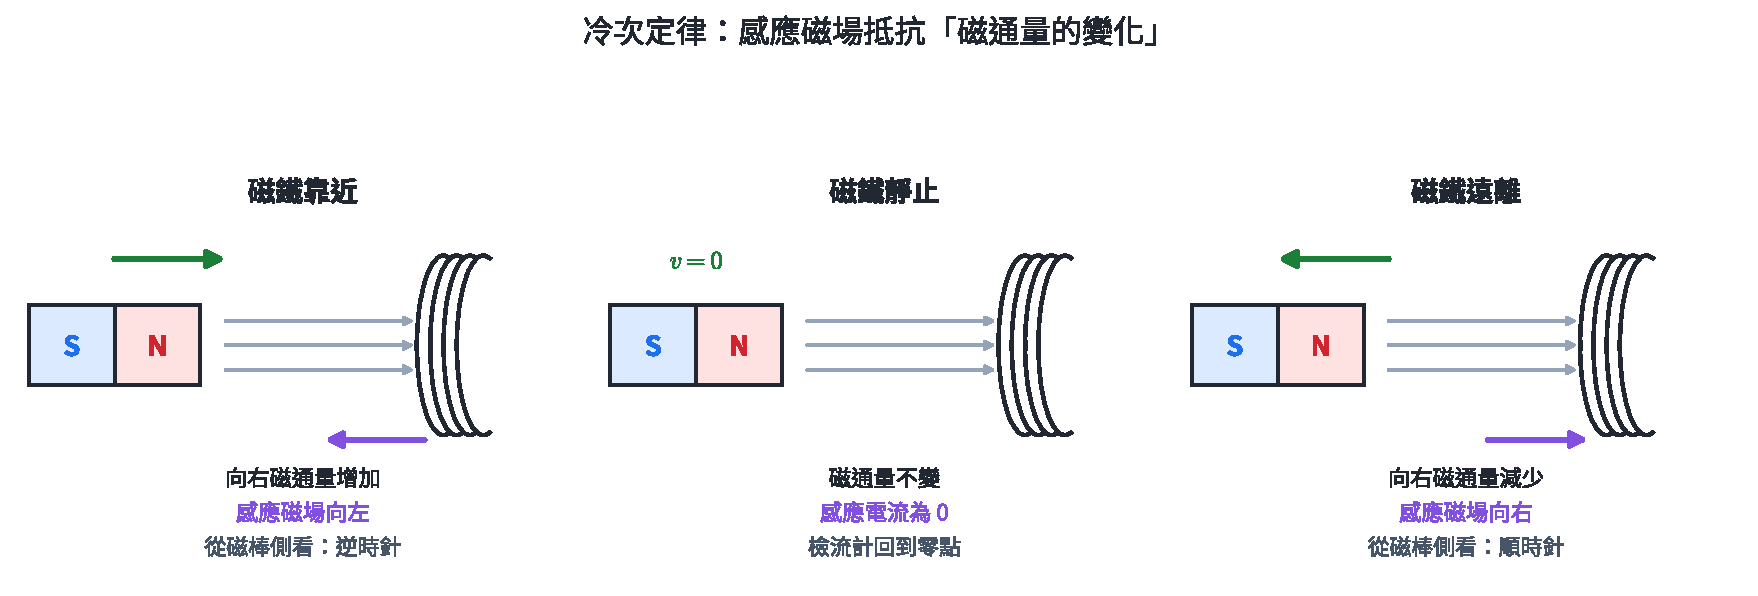
\includegraphics[width=0.96\linewidth,height=\textheight,keepaspectratio,alt={圖 3｜N 極靠近時線圈近端形成 N 極以排斥；停止時磁通量不變；遠離時近端形成 S 極以吸引。}]{assets/必物-4-電磁感應與冷次定律.pdf}
\caption{圖 3｜N 極靠近時線圈近端形成 N 極以排斥；停止時磁通量不變；遠離時近端形成 S 極以吸引。}
\end{figure}

方向判定可分成三步：

\begin{enumerate}
\def\labelenumi{\arabic{enumi}.}
\tightlist
\item
  指出原磁場穿過線圈的方向。
\item
  判定原磁通量正在增加或減少。
\item
  讓感應磁場抵抗這項變化，再用線圈右手定則換成感應電流方向。
\end{enumerate}

冷次定律的「抵抗變化」也符合能量守恆。若磁鐵靠近時線圈反而吸引磁鐵，磁鐵會自行越來越快，同時又產生電能；能量將無來源地增加。實際上，線圈的感應磁力阻礙相對運動，外力必須做功，機械能才轉成電能與熱。

\begin{HandoutWorkedExample}

\subsection{完整示範 4｜磁鐵靠近與遠離線圈}\label{ux5b8cux6574ux793aux7bc4-4ux78c1ux9435ux9760ux8fd1ux8207ux9060ux96e2ux7ddaux5708}

條形磁鐵的 N 極朝向線圈，沿線圈軸靠近。從磁鐵一側看線圈，求感應電流方向；再判斷磁鐵遠離時的方向。

\textbf{靠近：}N 極在靠近線圈處建立指向遠離 N 極的磁場，穿過線圈的磁通量增加。線圈近端形成 N 極來抵抗靠近。從磁鐵側看，近端為 N 極需要電流逆時針。

\textbf{遠離：}原方向磁通量減少。線圈建立同方向磁場以補償減少，近端形成 S 極吸引離開的 N 極。從磁鐵側看，電流改為順時針。

\textbf{停止：}磁鐵位置固定後，磁通量不再改變，感應電動勢降為零。

\end{HandoutWorkedExample}

\begin{HandoutWorkedExample}

\subsection{完整示範 5｜矩形線圈進出有限磁場區}\label{ux5b8cux6574ux793aux7bc4-5ux77e9ux5f62ux7ddaux5708ux9032ux51faux6709ux9650ux78c1ux5834ux5340}

矩形線圈以固定速度向右移動，進入一塊磁場穿出紙面的區域。

\textbf{進入階段：}線圈與磁場區重疊面積增加，穿出紙面的磁通量增加。感應磁場指向紙面內，感應電流為順時針。

\textbf{完全位於均勻磁場區：}\(B\)、線圈面積與方向都固定，穿過整個線圈的磁通量不變，感應電流為零。

\textbf{離開階段：}穿出紙面的磁通量減少。感應磁場指向紙面外，感應電流為逆時針。

三個階段的差異由 \(\Delta\Phi_B/\Delta t\) 決定；線圈是否正在移動本身不足以決定感應電流。

\end{HandoutWorkedExample}

\subsection{2.3 發電、變壓與近距離能量傳輸}\label{ux767cux96fbux8b8aux58d3ux8207ux8fd1ux8dddux96e2ux80fdux91cfux50b3ux8f38}

\begin{figure}
\centering
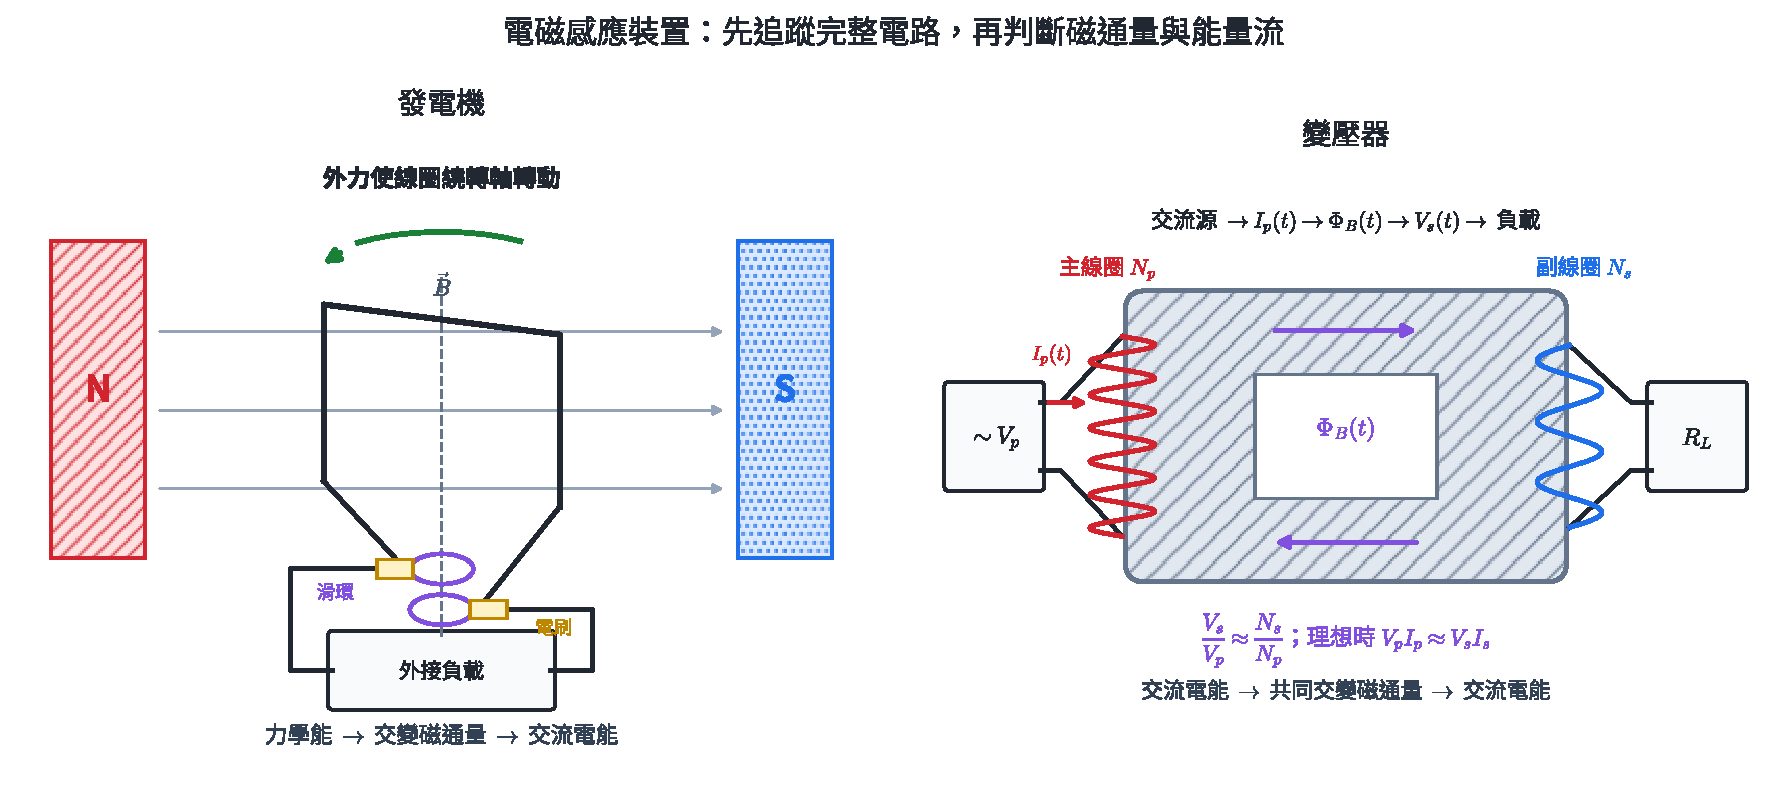
\includegraphics[width=0.96\linewidth,height=\textheight,keepaspectratio,alt={圖 4｜發電機線圈的兩端經滑環、電刷與負載閉合；變壓器的初級接交流源、次級接負載，兩個電路由共同交變磁通量耦合。}]{assets/必物-4-發電機與變壓器.pdf}
\caption{圖 4｜發電機線圈的兩端經滑環、電刷與負載閉合；變壓器的初級接交流源、次級接負載，兩個電路由共同交變磁通量耦合。}
\end{figure}

\subsubsection{發電機}\label{ux767cux96fbux6a5f}

線圈在磁場中轉動時，\(\theta\) 持續改變，所以磁通量週期性改變，輸出交流電。水力、風力與火力發電的上游能源不同，發電機的共同核心都是讓線圈與磁場相對轉動，把機械能轉成電能。

\subsubsection{變壓器}\label{ux8b8aux58d3ux5668}

初級線圈通入交流電，鐵芯中的磁通量持續改變，次級線圈因而產生感應電動勢。理想變壓器滿足

\[
\frac{V_s}{V_p}\approx\frac{N_s}{N_p},
\qquad
V_pI_p\approx V_sI_s.
\]

升高電壓會相應降低電流。在輸電功率固定時，線路熱損耗近似為 \(P_{\text{loss}}=I^2R\)；先升壓、降低電流，可顯著減少長距離輸電損耗。真實變壓器另有線圈電阻、漏磁與渦電流損失，輸出功率小於輸入功率。

\subsubsection{感應爐與無線充電}\label{ux611fux61c9ux7210ux8207ux7121ux7ddaux5145ux96fb}

感應爐線圈中的交流電建立快速變動磁場，使鍋底產生渦電流並以電阻熱升溫。無線充電的發射線圈建立交變磁場，接收線圈取得感應電動勢，再經整流與控制電路供電。兩線圈距離增加或方向偏離時，能穿過接收線圈的交變磁通量通常減少，傳能效率下降。

\begin{HandoutWorkedExample}

\subsection{完整示範 6｜理想變壓器的匝數比}\label{ux5b8cux6574ux793aux7bc4-6ux7406ux60f3ux8b8aux58d3ux5668ux7684ux531dux6578ux6bd4}

理想變壓器初級線圈 \(N_p=500\) 匝、次級線圈 \(N_s=50\) 匝，初級交流電壓為 \(110\ \mathrm V\)。求次級電壓。

\[
\frac{V_s}{110}=\frac{50}{500}=0.10
\quad\Rightarrow\quad
V_s=11\ \mathrm V.
\]

這是一個降壓變壓器。若次級輸出電流為 \(2.0\ \mathrm A\)，理想功率守恆給出

\[
I_p=\frac{V_sI_s}{V_p}
=\frac{(11)(2.0)}{110}
=0.20\ \mathrm A.
\]

變壓器需要變動磁通量，穩定直流只在接通或切斷的短暫過程產生感應。

\end{HandoutWorkedExample}

\subsection{2.4 家庭用電的並聯與保護}\label{ux5bb6ux5eadux7528ux96fbux7684ux4e26ux806fux8207ux4fddux8b77}

家庭電器接在並聯支路上，因此各支路獲得相同額定電壓，也能獨立開關。圖 5 把火線、電器、回線與保護元件放在同一條電流路徑上。

\begin{figure}
\centering
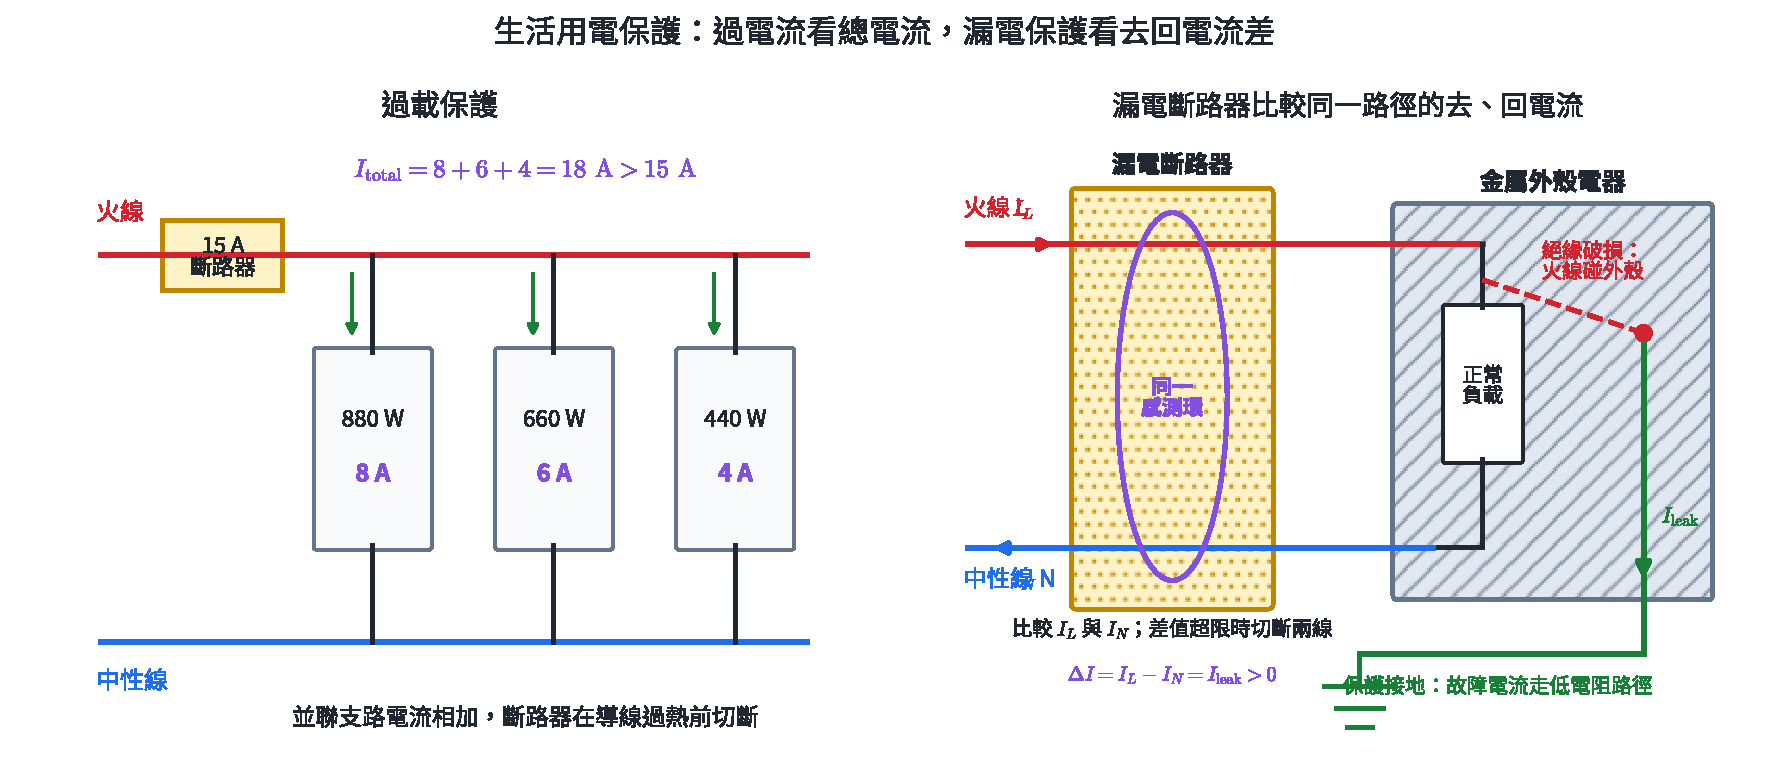
\includegraphics[width=0.96\linewidth,height=\textheight,keepaspectratio,alt={圖 5｜家用支路並聯；過電流保護裝在火線。漏電斷路器讓火線與中性線共同穿過感測環，比較去、回電流，保護接地線則不穿過感測環。}]{assets/必物-4-家用電路與保護.pdf}
\caption{圖 5｜家用支路並聯；過電流保護裝在火線。漏電斷路器讓火線與中性線共同穿過感測環，比較去、回電流，保護接地線則不穿過感測環。}
\end{figure}

在額定電壓 \(V\) 下，電器功率 \(P\) 與電流近似滿足

\[
P=VI,
\qquad
I=\frac{P}{V}.
\]

同一支路同時使用多個電器時，總電流是各電器電流相加。導線的發熱率近似 \(I^2R\)，所以過載會讓溫度快速上升。

\begin{itemize}
\tightlist
\item
  \textbf{保險絲或無熔絲開關}：電流超過額定值時切斷火線，處理過載與短路。
\item
  \textbf{接地線}：金屬外殼若意外帶電，提供低電阻故障電流路徑，使保護裝置快速動作，並降低人體承受的接觸電壓。
\item
  \textbf{漏電斷路器}：比較流出與流回的電流；若差值表示部分電流經其他路徑流走，就快速斷電。
\item
  \textbf{乾燥絕緣與完整外皮}：提高人體與外界間的電阻，降低通過人體的電流。
\end{itemize}

\begin{HandoutWorkedExample}

\subsection{完整示範 7｜延長線是否過載}\label{ux5b8cux6574ux793aux7bc4-7ux5ef6ux9577ux7ddaux662fux5426ux904eux8f09}

\(110\ \mathrm V\) 的延長線額定電流為 \(15\ \mathrm A\)，同時接上 \(1100\ \mathrm W\) 電熱器與 \(880\ \mathrm W\) 吹風機。求總電流並判斷。

\[
I_{\text{總}}
=\frac{1100+880}{110}
=18.0\ \mathrm A.
\]

\(18.0\ \mathrm A\) 超過額定 \(15\ \mathrm A\)，導線發熱率也會因 \(I^2\) 顯著上升。這組合屬於過載，應改用容量足夠且分屬合適支路的供電方式。

短路則是火線與回線之間出現極低電阻路徑，電流可在很短時間內急遽增加；過電流保護裝置必須快速切斷。

\end{HandoutWorkedExample}

\begin{HandoutSelfCheck}

\subsection{本節獨立練習}\label{ux672cux7bc0ux7368ux7acbux7df4ux7fd2-1}

\begin{enumerate}
\def\labelenumi{\arabic{enumi}.}
\tightlist
\item
  線圈固定不動，但磁場由 \(0.20\ \mathrm T\) 均勻增至 \(0.50\ \mathrm T\)。線圈中是否可能產生感應電動勢？指出原因。
\item
  磁鐵 N 極由線圈上方向下靠近。從磁鐵側看，線圈上表面要形成哪一磁極？感應電流為順時針或逆時針？
\item
  線圈完全位於均勻磁場內並以固定速度平移，面積與方向不變。感應電動勢為何？
\item
  變壓器初級接穩定直流後，為何次級只在接通瞬間可能出現短暫訊號？
\item
  \(110\ \mathrm V\) 支路同時使用 \(770\ \mathrm W\) 與 \(990\ \mathrm W\) 電器。總電流是多少？是否超過 \(15\ \mathrm A\)？
\item
  金屬外殼電器若絕緣損壞，接地線與漏電斷路器各提供哪一層保護？
\end{enumerate}

\textbf{簡答：}1. 可能，因 \(B\) 改變使磁通量改變。2. 上表面形成 N 極，從上看為逆時針。3. 磁通量固定，感應電動勢為零。4. 接通瞬間電流與磁通量正在改變，穩定後磁通量固定。5. \(I=(770+990)/110=16.0\ \mathrm A\)，超過。6. 接地線提供低電阻故障路徑；漏電斷路器偵測去回電流差並切斷電源。

\end{HandoutSelfCheck}

\section{3. 電場與磁場共同形成電磁波}\label{ux96fbux5834ux8207ux78c1ux5834ux5171ux540cux5f62ux6210ux96fbux78c1ux6ce2}

\subsection{3.1 從四類實驗規律到電磁波}\label{ux5f9eux56dbux985eux5be6ux9a57ux898fux5f8bux5230ux96fbux78c1ux6ce2}

十九世紀的電磁實驗可整理成四項互相銜接的規律：

{\def\LTcaptype{none} % do not increment counter
\begin{longtable}[]{@{}
  >{\raggedright\arraybackslash}p{(\linewidth - 4\tabcolsep) * \real{0.3333}}
  >{\raggedright\arraybackslash}p{(\linewidth - 4\tabcolsep) * \real{0.3333}}
  >{\raggedright\arraybackslash}p{(\linewidth - 4\tabcolsep) * \real{0.3333}}@{}}
\toprule\noalign{}
\begin{minipage}[b]{\linewidth}\raggedright
實驗規律
\end{minipage} & \begin{minipage}[b]{\linewidth}\raggedright
可觀察的現象
\end{minipage} & \begin{minipage}[b]{\linewidth}\raggedright
形成的連結
\end{minipage} \\
\midrule\noalign{}
\endhead
\bottomrule\noalign{}
\endlastfoot
電荷建立電場 & 帶電體使周圍測試電荷受力 & 電荷 \(\rightarrow\) 電場 \\
電流建立磁場 & 通電導線使磁針偏轉 & 移動電荷 \(\rightarrow\) 磁場 \\
變動磁場建立渦旋電場 & 線圈磁通量改變而感應出電動勢 & 變動磁場 \(\rightarrow\) 電場 \\
變動電場也建立磁場 & 電容器充放電時，周圍磁場仍連續 & 變動電場 \(\rightarrow\) 磁場 \\
\end{longtable}
}

馬克士威把這些關係合成電磁理論。他的關鍵預測是：一旦空間中出現變動電場，它能建立變動磁場；變動磁場又建立電場，因此擾動可以離開原來的電荷，在空間中向外傳播。

\begin{figure}
\centering
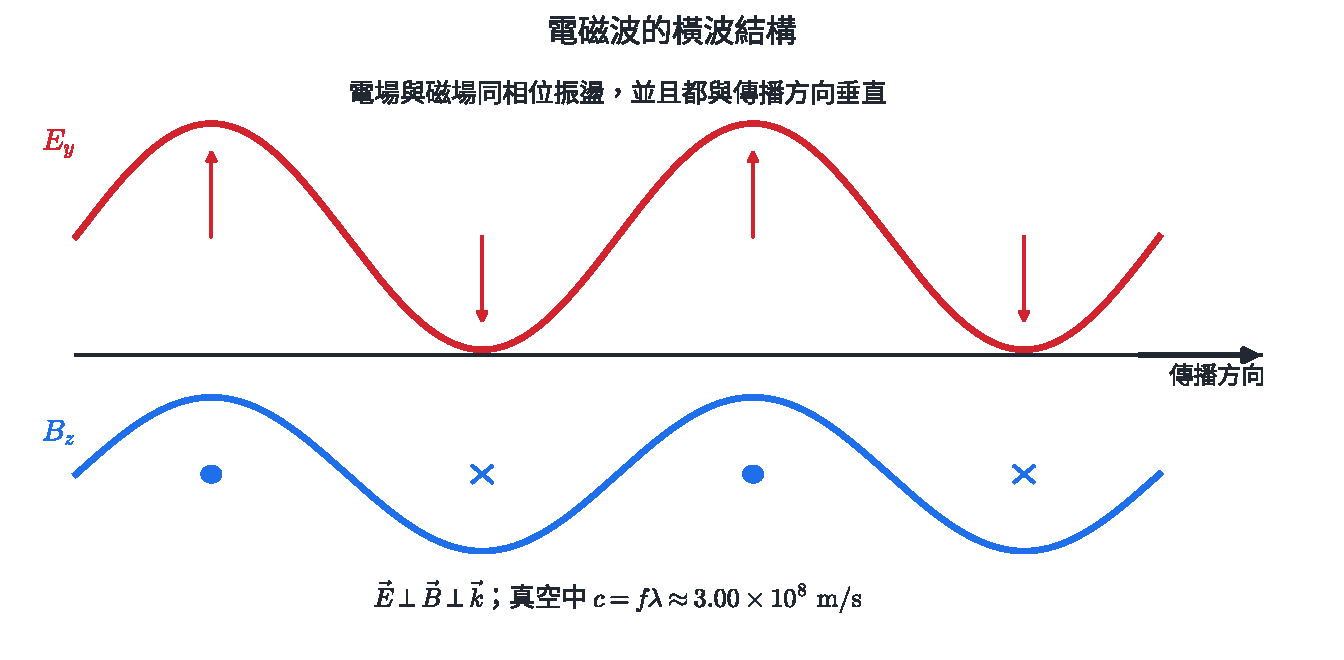
\includegraphics[width=0.94\linewidth,height=\textheight,keepaspectratio,alt={圖 6｜平面電磁波中，電場、磁場與傳播方向彼此垂直，且電場與磁場同相。}]{assets/必物-4-電磁波正交結構.pdf}
\caption{圖 6｜平面電磁波中，電場、磁場與傳播方向彼此垂直，且電場與磁場同相。}
\end{figure}

在真空中，電磁波的傳播速率為

\[
c\approx3.00\times10^8\ \mathrm{m/s},
\]

並滿足所有週期波共有的關係

\[
c=f\lambda.
\]

圖 6 中 \(\vec E\)、\(\vec B\) 與傳播方向兩兩垂直；傳播方向與 \(\vec E\times\vec B\) 同向。電場與磁場在同一位置同時達到最大、同時過零，稱為同相。電磁波不需要物質介質，因此能穿越真空；它攜帶能量與動量，天線、太陽能板與遙測器都利用這項性質。

發射天線中的電荷來回振盪，建立同頻率的變動電場與磁場；接收天線中的自由電荷受外來電場推動，形成可被電路分析的交流訊號。資訊可藉由調整載波的振幅、頻率或相位編碼。

\begin{HandoutWorkedExample}

\subsection{完整示範 8｜廣播波的波長}\label{ux5b8cux6574ux793aux7bc4-8ux5ee3ux64adux6ce2ux7684ux6ce2ux9577}

一座發射台以 \(100\ \mathrm{MHz}\) 的頻率發射電磁波。求真空中的波長。

先換單位：

\[
100\ \mathrm{MHz}=1.00\times10^8\ \mathrm{Hz}.
\]

再用 \(c=f\lambda\)：

\[
\lambda=\frac{c}{f}
=\frac{3.00\times10^8}{1.00\times10^8}
=3.00\ \mathrm m.
\]

天線尺寸通常會和波長的某個比例有關，因此不同頻段需要不同的天線結構。

\end{HandoutWorkedExample}

\subsection{3.2 電磁波譜}\label{ux96fbux78c1ux6ce2ux8b5c}

不同頻率的電磁波本質相同，差別在頻率、波長及它與物質互動的方式。圖 7 同時排列波長與頻率：往右頻率增加，波長減少。

\begin{figure}
\centering
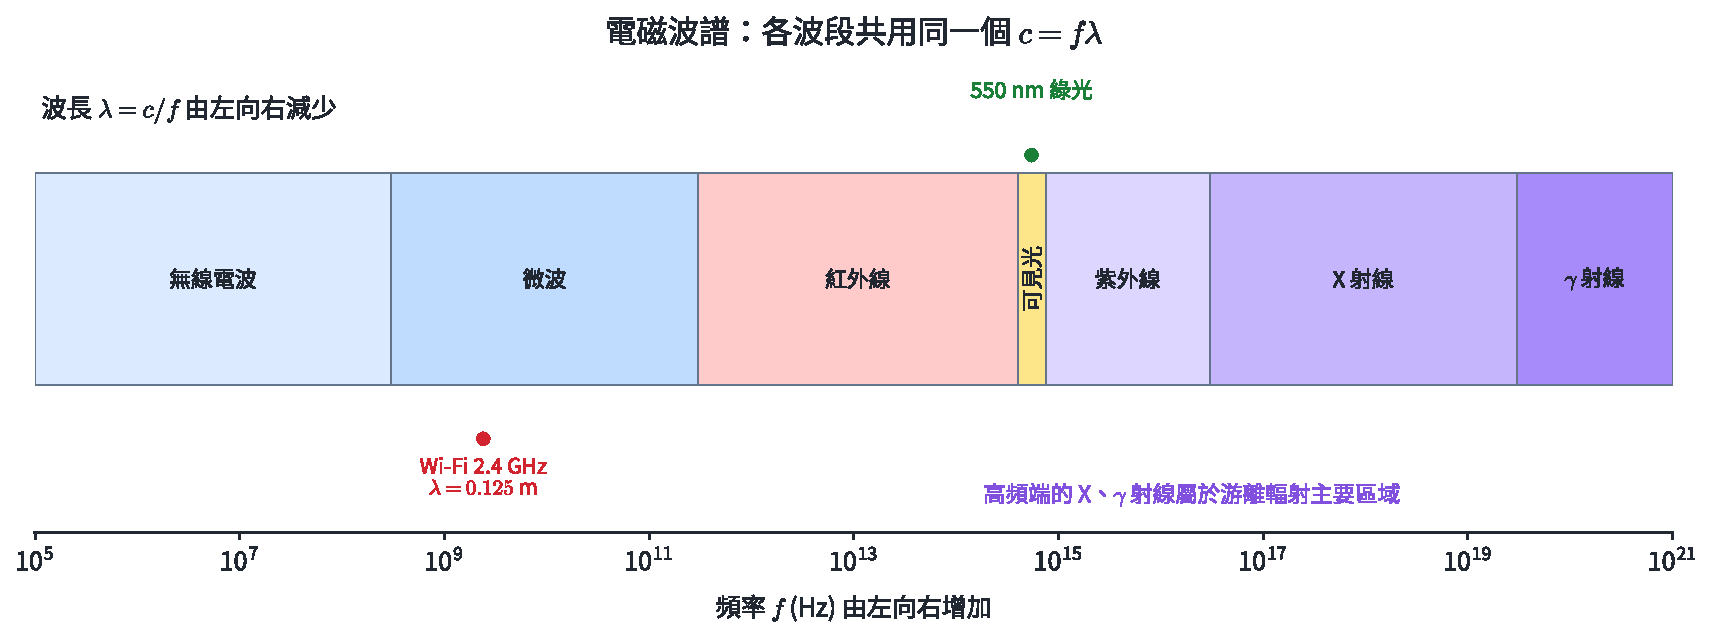
\includegraphics[width=0.98\linewidth,height=\textheight,keepaspectratio,alt={圖 7｜電磁波由無線電波、微波、紅外線、可見光、紫外線、X 射線到伽瑪射線；頻率向右增加。}]{assets/必物-4-電磁波譜.pdf}
\caption{圖 7｜電磁波由無線電波、微波、紅外線、可見光、紫外線、X 射線到伽瑪射線；頻率向右增加。}
\end{figure}

{\def\LTcaptype{none} % do not increment counter
\begin{longtable}[]{@{}
  >{\raggedright\arraybackslash}p{(\linewidth - 4\tabcolsep) * \real{0.3333}}
  >{\raggedright\arraybackslash}p{(\linewidth - 4\tabcolsep) * \real{0.3333}}
  >{\raggedright\arraybackslash}p{(\linewidth - 4\tabcolsep) * \real{0.3333}}@{}}
\toprule\noalign{}
\begin{minipage}[b]{\linewidth}\raggedright
波段
\end{minipage} & \begin{minipage}[b]{\linewidth}\raggedright
常見來源或用途
\end{minipage} & \begin{minipage}[b]{\linewidth}\raggedright
與物質互動的重點
\end{minipage} \\
\midrule\noalign{}
\endhead
\bottomrule\noalign{}
\endlastfoot
無線電波 & 廣播、行動通訊、無線感測 & 天線中的電荷集體振盪 \\
微波 & 雷達、衛星通訊、微波加熱 & 可驅動極性分子的轉動與介電損耗 \\
紅外線 & 熱像、遙控器、溫度感測 & 常與分子振動及熱輻射相關 \\
可見光 & 視覺、照明、光纖、顯微鏡 & 眼睛與感光元件可偵測 \\
紫外線 & 殺菌、螢光、材料分析 & 單一光子能量較高，可造成化學反應與皮膚傷害 \\
X 射線 & 醫學成像、材料檢測 & 穿透軟組織能力較強，屬游離輻射 \\
伽瑪射線 & 核醫、放射治療、天文觀測 & 光子能量極高，屬游離輻射 \\
\end{longtable}
}

光子的能量與頻率關係為 \(E=hf\)；同一波段的危害仍取決於強度、照射時間與吸收情況。紫外線、X 射線及伽瑪射線的單一光子能量較高，能使原子或分子游離；射頻與微波通常以加熱等非游離作用為主。安全判斷要結合頻率與暴露量。

\begin{HandoutWorkedExample}

\subsection{完整示範 9｜Wi‑Fi 訊號的波長與能量類型}\label{ux5b8cux6574ux793aux7bc4-9wifi-ux8a0aux865fux7684ux6ce2ux9577ux8207ux80fdux91cfux985eux578b}

\(2.4\ \mathrm{GHz}\) 的無線訊號在空氣中近似以光速傳播：

\[
\lambda=\frac{3.00\times10^8}{2.4\times10^9}
=1.25\times10^{-1}\ \mathrm m
=12.5\ \mathrm{cm}.
\]

它位於微波範圍。其單一光子能量遠低於 X 射線，屬非游離電磁波；實際吸收能量仍受發射功率、距離、時間與人體組織耦合情況影響。

\end{HandoutWorkedExample}

\begin{HandoutWorkedExample}

\subsection{完整示範 10｜綠光進入玻璃後哪些量改變}\label{ux5b8cux6574ux793aux7bc4-10ux7da0ux5149ux9032ux5165ux73bbux7483ux5f8cux54eaux4e9bux91cfux6539ux8b8a}

真空波長為 \(550\ \mathrm{nm}\) 的綠光，其頻率為

\[
f=\frac{c}{\lambda}
=\frac{3.00\times10^8}{550\times10^{-9}}
\approx5.45\times10^{14}\ \mathrm{Hz}.
\]

光進入玻璃時，邊界兩側的振動必須保持連續，所以\textbf{頻率由光源決定並保持不變}。玻璃中的速率比真空小，依 \(v=f\lambda\)，玻璃中的波長也按相同比例縮短。

顏色通常對應頻率；介質中的波長改變不代表光源頻率改變。

\end{HandoutWorkedExample}

\begin{HandoutSelfCheck}

\subsection{本節獨立練習}\label{ux672cux7bc0ux7368ux7acbux7df4ux7fd2-2}

\begin{enumerate}
\def\labelenumi{\arabic{enumi}.}
\tightlist
\item
  平面電磁波向東傳播，某時某處電場向上。若取東、北、上分別為 \(+x,+y,+z\)，磁場應指向哪個方向，才能使 \(\vec E\times\vec B\) 向東？
\item
  \(300\ \mathrm{MHz}\) 電磁波在真空中的波長是多少？
\item
  依頻率由低到高排列：紅外線、X 射線、無線電波、紫外線。
\item
  同一束光由真空進入玻璃，速率變為 \(0.67c\)。頻率與波長各如何改變？
\item
  說明接收天線如何把遠方的電磁波轉成電路訊號。
\end{enumerate}

\textbf{簡答：}1. 向南，即 \(-y\)，因 \(+z\times(-y)=+x\)。2. \(1.00\ \mathrm m\)。3. 無線電波、紅外線、紫外線、X 射線。4. 頻率不變，波長變為原來 \(0.67\) 倍。5. 電磁波的電場驅動天線內自由電荷振盪，形成同頻交流訊號。

\end{HandoutSelfCheck}

\section{4. 光的波動證據與週期波}\label{ux5149ux7684ux6ce2ux52d5ux8b49ux64daux8207ux9031ux671fux6ce2}

\subsection{4.1 光的模型如何由證據篩選}\label{ux5149ux7684ux6a21ux578bux5982ux4f55ux7531ux8b49ux64daux7be9ux9078}

光沿直線傳播並能反射，早期的微粒模型可以描述這些現象；惠更斯的波動模型則用波前解釋反射與折射。兩個模型對折射介質中的光速給出不同預測：

\begin{itemize}
\tightlist
\item
  古典微粒模型假設光粒進入光密介質後加速。
\item
  波動模型預測光進入光密介質後速率降低。
\end{itemize}

楊氏雙狹縫實驗出現規律明暗條紋，直接顯示疊加與干涉；傅科後來測得光在水中比在空氣中慢，支持波動模型的折射預測。馬克士威再指出光是電磁波。現代實驗也顯示光的能量交換具有光子特徵；波動與粒子描述分別對應不同測量情境，本章以波動模型處理傳播與光路。

證據的角色可以整理為：

{\def\LTcaptype{none} % do not increment counter
\begin{longtable}[]{@{}ll@{}}
\toprule\noalign{}
證據 & 支持的模型內容 \\
\midrule\noalign{}
\endhead
\bottomrule\noalign{}
\endlastfoot
影子與小孔成像 & 波長相對孔徑很小時，光近似直線傳播 \\
反射與折射 & 波前在邊界的幾何演化 \\
雙狹縫明暗條紋 & 兩列相干波的疊加 \\
單狹縫展寬 & 有限孔徑造成繞射 \\
水中光速較慢 & 折射率 \(n=c/v>1\) 的波動描述 \\
光電效應等能量交換 & 光子能量以 \(E=hf\) 為單位交換 \\
\end{longtable}
}

\subsection{4.2 一張圖分清介質質點與波形}\label{ux4e00ux5f35ux5716ux5206ux6e05ux4ecbux8ceaux8ceaux9edeux8207ux6ce2ux5f62}

圖 8 上圖固定同一時刻，比較不同位置的位移，因此可量出波長；下圖固定質點 \(P\) 的位置，追蹤它隨時間的位移，因此可量出週期。波向右傳時，質點 \(P\) 只在平衡位置附近上下振動，波形與能量向右傳播。

\begin{figure}
\centering
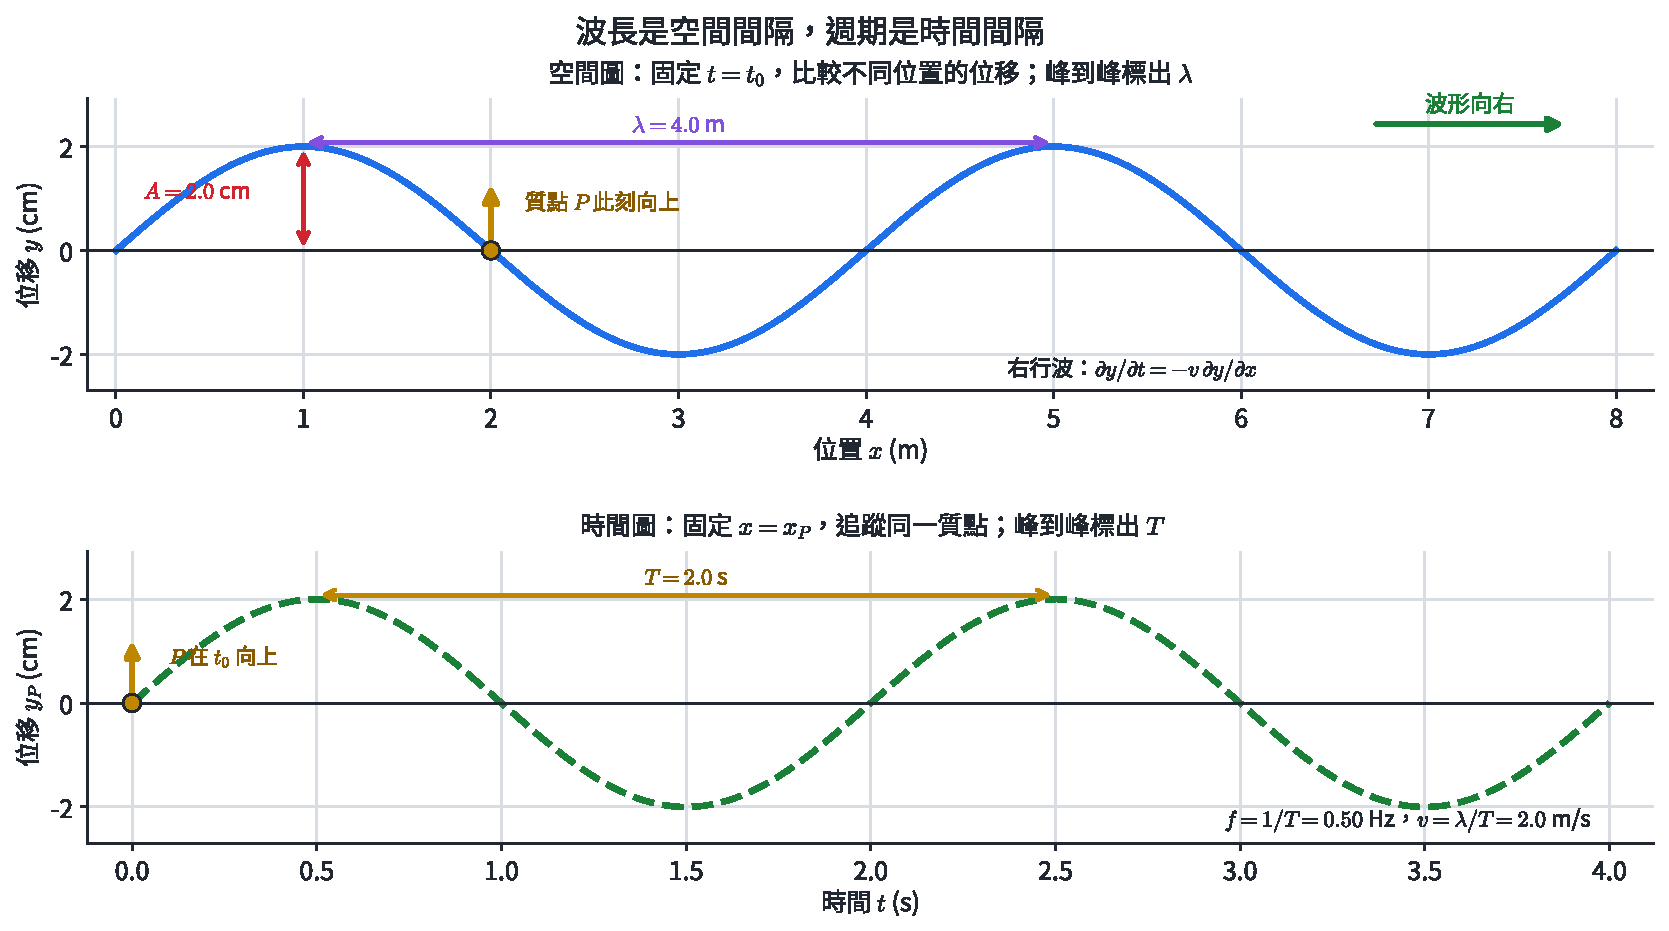
\includegraphics[width=0.96\linewidth,height=\textheight,keepaspectratio,alt={圖 8｜空間圖的峰到峰距離是波長 \textbackslash lambda，時間圖的峰到峰時間是週期 T；右行波在負斜率處的質點向上。}]{assets/必物-4-週期波參數與質點運動.pdf}
\caption{圖 8｜空間圖的峰到峰距離是波長 \(\lambda\)，時間圖的峰到峰時間是週期 \(T\)；右行波在負斜率處的質點向上。}
\end{figure}

\begin{itemize}
\tightlist
\item
  \textbf{振幅 \(A\)}：質點離平衡位置的最大位移，反映振動強弱。
\item
  \textbf{週期 \(T\)}：同一質點完成一次振動所需時間。
\item
  \textbf{頻率 \(f\)}：每秒完成的振動次數，\(f=1/T\)。
\item
  \textbf{波長 \(\lambda\)}：同一時刻，相鄰同相位點的距離，例如波峰到下一個波峰。
\item
  \textbf{波速 \(v\)}：波形或相位向前傳播的速率，由介質性質決定。
\end{itemize}

一個週期 \(T\) 內，波形前進一個波長 \(\lambda\)，所以

\[
v=\frac{\lambda}{T}=f\lambda.
\]

這條式子的因果結構很重要：波源決定頻率，介質決定波速；同一波源進入另一介質時，頻率保持不變，波長隨波速改變。

對向右傳的橫波，可把波形想成整體向右平移。若某點右側的波形較低，稍後這段較高的波形會移到該點，因此該點正向上運動。用數學寫成

\[
\frac{\partial y}{\partial t}=-v\frac{\partial y}{\partial x}.
\]

因此右行波在\textbf{負斜率}處質點向上，在\textbf{正斜率}處質點向下；波峰與波谷當下速度為零，但下一瞬間的運動方向由附近曲率與回復力決定。

\begin{HandoutWorkedExample}

\subsection{完整示範 11｜由週期與波長求波速}\label{ux5b8cux6574ux793aux7bc4-11ux7531ux9031ux671fux8207ux6ce2ux9577ux6c42ux6ce2ux901f}

水面波相鄰波峰距離為 \(1.2\ \mathrm m\)，固定浮標每 \(0.40\ \mathrm s\) 完成一次上下振動。

\[
\lambda=1.2\ \mathrm m,\qquad
T=0.40\ \mathrm s,
\]

所以

\[
f=\frac1T=2.5\ \mathrm{Hz},
\qquad
v=f\lambda=(2.5)(1.2)=3.0\ \mathrm{m/s}.
\]

浮標並未以 \(3.0\ \mathrm{m/s}\) 向前漂移；這個速度描述波形與能量的傳播。

\end{HandoutWorkedExample}

\begin{HandoutWorkedExample}

\subsection{完整示範 12｜由波形斜率判斷質點方向}\label{ux5b8cux6574ux793aux7bc4-12ux7531ux6ce2ux5f62ux659cux7387ux5224ux65b7ux8ceaux9edeux65b9ux5411}

某橫波向右傳。時刻 \(t_0\)，質點 P 位於平衡位置，波形在 P 處由左上往右下，斜率為負。

波形稍後整體右移，P 左側原本較高的部分會到達 P，因此 P 的位移將增加，當下速度向上。也可用

\[
\frac{\partial y}{\partial t}=-v\frac{\partial y}{\partial x}
\]

判斷：\(v>0\) 且空間斜率為負，所以時間變化率為正。

\end{HandoutWorkedExample}

\begin{HandoutWorkedExample}

\subsection{完整示範 13｜跨介質後的波長}\label{ux5b8cux6574ux793aux7bc4-13ux8de8ux4ecbux8ceaux5f8cux7684ux6ce2ux9577}

頻率 \(5.0\ \mathrm{Hz}\) 的水波由深水區進入淺水區，波速由 \(4.0\ \mathrm{m/s}\) 降為 \(2.5\ \mathrm{m/s}\)。

入射區：

\[
\lambda_1=\frac{v_1}{f}=\frac{4.0}{5.0}=0.80\ \mathrm m.
\]

折射區：

\[
\lambda_2=\frac{v_2}{f}=\frac{2.5}{5.0}=0.50\ \mathrm m.
\]

頻率保持 \(5.0\ \mathrm{Hz}\)，因為邊界上的波峰到達節奏必須連續；淺水區波速較小，所以波前間距縮短。

\end{HandoutWorkedExample}

\begin{HandoutSelfCheck}

\subsection{本節獨立練習}\label{ux672cux7bc0ux7368ux7acbux7df4ux7fd2-3}

\begin{enumerate}
\def\labelenumi{\arabic{enumi}.}
\tightlist
\item
  波的週期為 \(0.25\ \mathrm s\)，求頻率。
\item
  波速為 \(12\ \mathrm{m/s}\)、頻率為 \(3.0\ \mathrm{Hz}\)，求波長。
\item
  右行橫波在某點的波形斜率為正。該質點當下向上或向下？
\item
  同一波源的波由介質 A 進入介質 B，波速變為原來一半。頻率與波長各如何改變？
\item
  楊氏雙狹縫與傅科水中測速，各排除了古典光模型的哪一項困難？
\end{enumerate}

\textbf{簡答：}1. \(4.0\ \mathrm{Hz}\)。2. \(4.0\ \mathrm m\)。3. 向下。4. 頻率不變，波長變為一半。5. 雙狹縫顯示穩定干涉，需用疊加解釋；水中光速較慢符合波動折射模型，與古典微粒模型的加速預測相反。

\end{HandoutSelfCheck}

\section{5. 反射、折射與惠更斯原理}\label{ux53cdux5c04ux6298ux5c04ux8207ux60e0ux66f4ux65afux539fux7406}

\subsection{5.1 光線、波前與法線}\label{ux5149ux7ddaux6ce2ux524dux8207ux6cd5ux7dda}

光線表示能量傳播方向，波前連接同相位的點；在均勻、各向同性介質中，光線垂直波前。圖 9 的所有角度都從邊界法線量起。

\begin{figure}
\centering
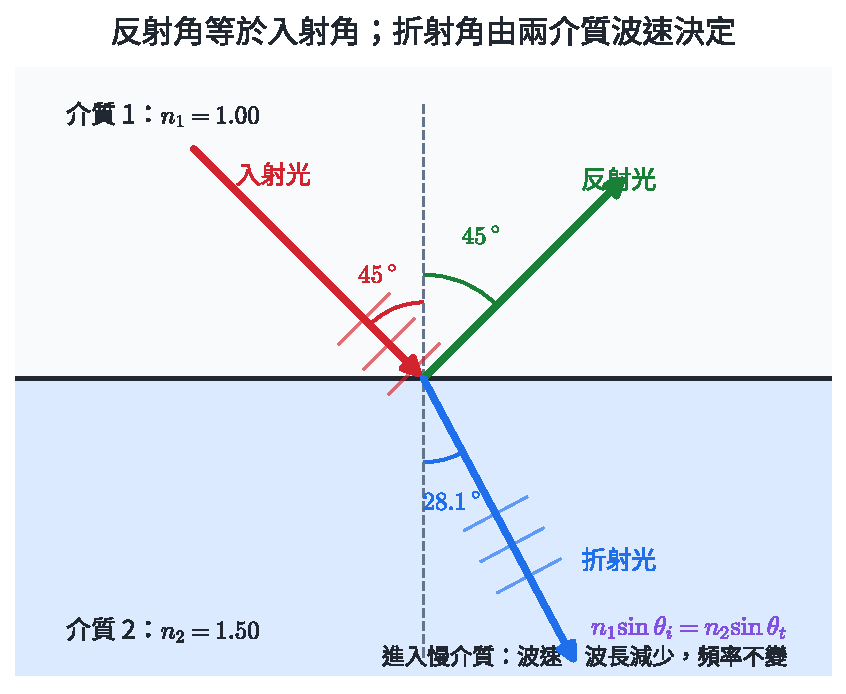
\includegraphics[width=0.96\linewidth,height=\textheight,keepaspectratio,alt={圖 9｜反射角等於入射角；光由空氣進入折射率 1.5 的玻璃，入射角 45\^{}\textbackslash circ 對應折射角約 28.1\^{}\textbackslash circ。}]{assets/必物-4-反射與折射光路.pdf}
\caption{圖 9｜反射角等於入射角；光由空氣進入折射率 1.5 的玻璃，入射角 \(45^\circ\) 對應折射角約 \(28.1^\circ\)。}
\end{figure}

反射定律為

\[
\theta_r=\theta_i.
\]

光由折射率 \(n_1\) 的介質進入 \(n_2\)，司乃耳定律為

\[
n_1\sin\theta_1=n_2\sin\theta_2,
\qquad
n=\frac{c}{v}.
\]

若 \(n_2>n_1\)，第二介質光速較小，折射角 \(\theta_2\) 較小，光線偏向法線；若 \(n_2<n_1\)，光線偏離法線。垂直入射時兩角都是 \(0^\circ\)，光路方向不轉折，但速率與波長仍會改變。

\begin{HandoutWorkedExample}

\subsection{完整示範 14｜由空氣射入玻璃}\label{ux5b8cux6574ux793aux7bc4-14ux7531ux7a7aux6c23ux5c04ux5165ux73bbux7483}

光由空氣射入折射率 \(1.50\) 的玻璃，入射角為 \(45.0^\circ\)，取空氣折射率為 \(1.00\)。

\[
(1.00)\sin45.0^\circ
=(1.50)\sin\theta_2,
\]

所以

\[
\sin\theta_2=\frac{\sin45.0^\circ}{1.50}
\approx0.4714,
\qquad
\theta_2\approx28.1^\circ.
\]

玻璃折射率較大，答案確實小於 \(45^\circ\)。玻璃內速率為 \(c/1.50\)，波長也變為真空波長的 \(1/1.50\)，頻率維持不變。

\end{HandoutWorkedExample}

\begin{HandoutWorkedExample}

\subsection{完整示範 15｜由光路比較介質}\label{ux5b8cux6574ux793aux7bc4-15ux7531ux5149ux8defux6bd4ux8f03ux4ecbux8cea}

同一束光由介質 A 射入介質 B，入射角 \(50^\circ\)，折射角 \(35^\circ\)。

由司乃耳定律，

\[
\frac{n_B}{n_A}
=\frac{\sin50^\circ}{\sin35^\circ}
\approx1.34.
\]

所以 \(n_B>n_A\)，且

\[
\frac{v_B}{v_A}=\frac{n_A}{n_B}\approx0.749.
\]

光在 B 中較慢，波長也較短。這組資料只決定 A、B 的相對折射率；若沒有其中一個介質的已知折射率，無法單獨求出兩者各自的 \(n\)。

\end{HandoutWorkedExample}

\subsection{5.2 惠更斯原理把波前推到下一時刻}\label{ux60e0ux66f4ux65afux539fux7406ux628aux6ce2ux524dux63a8ux5230ux4e0bux4e00ux6642ux523b}

\begin{figure}
\centering
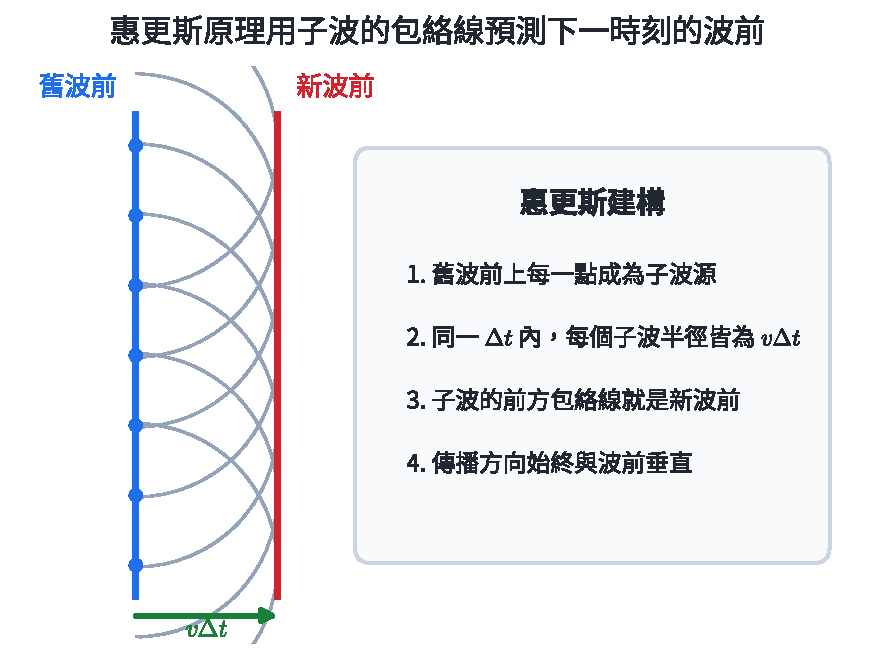
\includegraphics[width=0.96\linewidth,height=\textheight,keepaspectratio,alt={圖 10｜波前上每一點都產生次波；下一時刻所有次波的包絡面形成新波前。}]{assets/必物-4-惠更斯波前.pdf}
\caption{圖 10｜波前上每一點都產生次波；下一時刻所有次波的包絡面形成新波前。}
\end{figure}

惠更斯原理的操作方式是：

\begin{enumerate}
\def\labelenumi{\arabic{enumi}.}
\tightlist
\item
  把目前波前上的每一點視為次波源。
\item
  經過時間 \(\Delta t\)，每個次波在該介質中走過 \(v\Delta t\)。
\item
  所有次波最外側的共同包絡面形成下一個波前。
\end{enumerate}

在同一介質反射時，入射波前與反射波前在相同時間內走相同距離，幾何全等導出 \(\theta_i=\theta_r\)。

折射時，波前的一端先進入第二介質。取同一段時間 \(\Delta t\)：

\[
\text{介質 1 走過 }v_1\Delta t,
\qquad
\text{介質 2 走過 }v_2\Delta t.
\]

由波前幾何的兩個直角三角形，可得

\[
\frac{\sin\theta_1}{\sin\theta_2}
=\frac{v_1}{v_2}.
\]

再用 \(n=c/v\)：

\[
\frac{\sin\theta_1}{\sin\theta_2}
=\frac{n_2}{n_1}
\quad\Rightarrow\quad
n_1\sin\theta_1=n_2\sin\theta_2.
\]

這項推導顯示折射方向來自波前兩端速率不同；折射定律與波速改變是同一機制的兩種表達。

\begin{HandoutWorkedExample}

\subsection{完整示範 16｜由波速比判斷折射與波前密度}\label{ux5b8cux6574ux793aux7bc4-16ux7531ux6ce2ux901fux6bd4ux5224ux65b7ux6298ux5c04ux8207ux6ce2ux524dux5bc6ux5ea6}

平面波由介質 1 進入介質 2，介質 2 的波速為介質 1 的 \(2/3\)，入射角為 \(45^\circ\)。

頻率固定，因此

\[
\frac{\lambda_2}{\lambda_1}
=\frac{v_2}{v_1}
=\frac23.
\]

第二介質的波前間距變為原來 \(2/3\)，波前較密。由惠更斯幾何，

\[
\frac{\sin\theta_2}{\sin45^\circ}
=\frac{v_2}{v_1}
=\frac23,
\]

所以

\[
\sin\theta_2=\frac23\sin45^\circ\approx0.4714,
\qquad
\theta_2\approx28.1^\circ.
\]

波速降低，光線偏向法線；圖上波前也應同步變密。

\end{HandoutWorkedExample}

\begin{HandoutSelfCheck}

\subsection{本節獨立練習}\label{ux672cux7bc0ux7368ux7acbux7df4ux7fd2-4}

\begin{enumerate}
\def\labelenumi{\arabic{enumi}.}
\tightlist
\item
  光以相對法線 \(35^\circ\) 入射平面鏡，反射角是多少？入射光與反射光夾角是多少？
\item
  光由 \(n=1.50\) 的玻璃垂直射入空氣。傳播方向、頻率、速率與波長各如何改變？
\item
  光由空氣以 \(30^\circ\) 射入 \(n=1.50\) 玻璃，求折射角。
\item
  同一頻率的光在介質 A、B 中波長比 \(\lambda_A:\lambda_B=4:3\)。比較兩介質的波速與折射率。
\item
  用惠更斯原理說明光由快介質斜射入慢介質時，波前為何旋轉並使光線偏向法線。
\end{enumerate}

\textbf{簡答：}1. \(35^\circ\)；兩光線夾角為 \(70^\circ\)。2. 方向不變、頻率不變、速率增加、波長增加。3. \(\sin\theta_2=\sin30^\circ/1.50=1/3\)，\(\theta_2\approx19.5^\circ\)。4. \(v_A:v_B=4:3\)，\(n_A:n_B=3:4\)。5. 先進入慢介質的一端在同一時間走得較短，波前轉向；光線垂直波前，因而偏向法線。

\end{HandoutSelfCheck}

\clearpage

\section{6. 干涉與繞射}\label{ux5e72ux6d89ux8207ux7e5eux5c04}

\subsection{6.1 疊加、相位與路徑差}\label{ux758aux52a0ux76f8ux4f4dux8207ux8defux5f91ux5dee}

兩列波在同一位置相遇時，當下的總位移等於各列波位移的代數和。波通過後仍各自向前傳播，這是\textbf{疊加原理}。

\begin{figure}
\centering
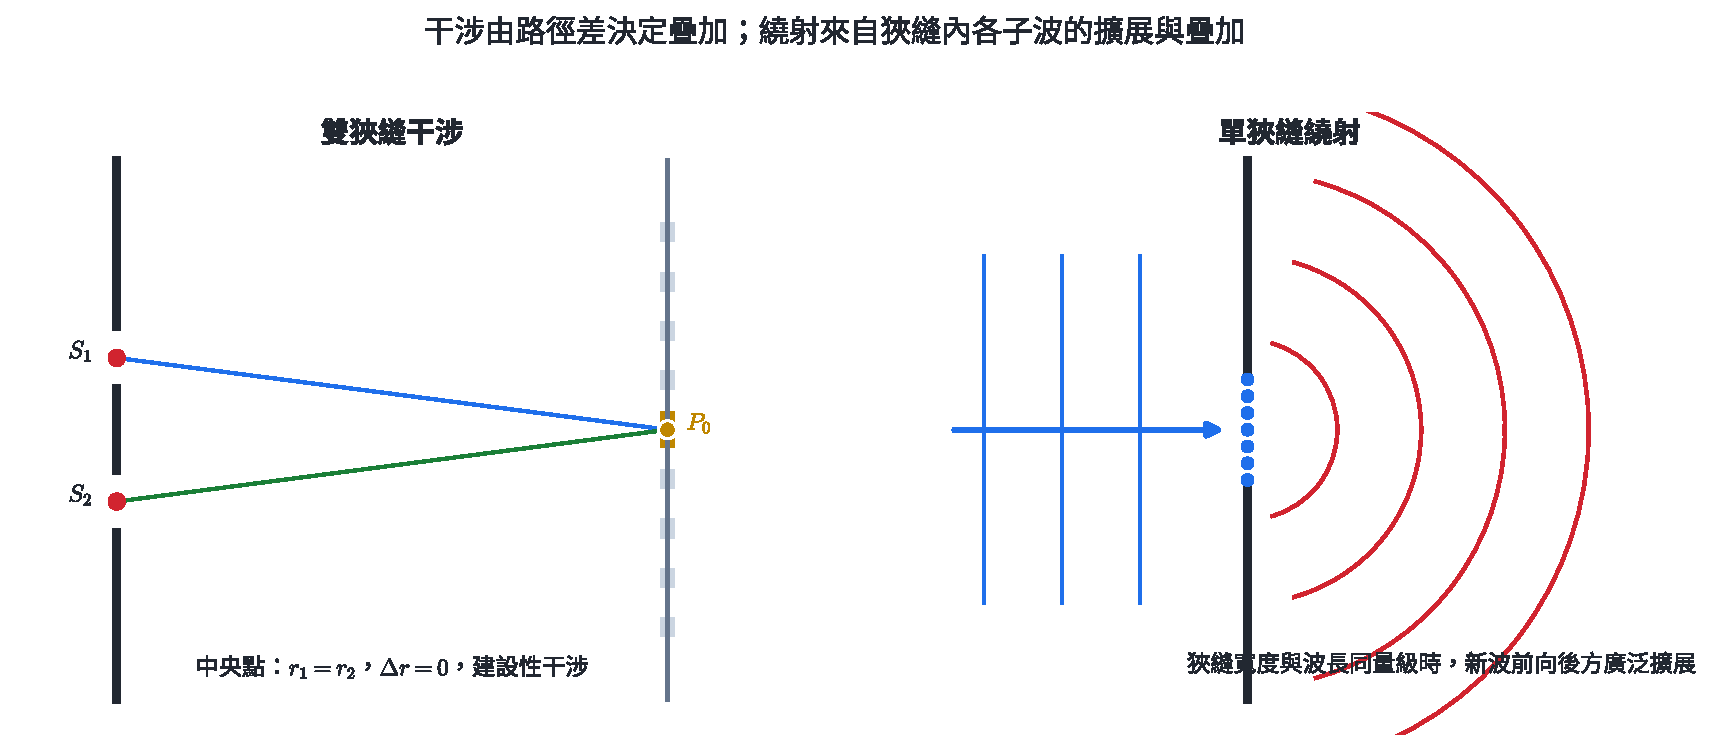
\includegraphics[width=0.96\linewidth,height=\textheight,keepaspectratio,alt={圖 11｜雙狹縫中央線兩路徑相等而形成亮紋；單狹縫寬度接近波長時，通過後明顯展開。}]{assets/必物-4-干涉與繞射.pdf}
\caption{圖 11｜雙狹縫中央線兩路徑相等而形成亮紋；單狹縫寬度接近波長時，通過後明顯展開。}
\end{figure}

兩個同頻率、相位差固定的波源稱為相干波源。雙狹縫由同一入射波照明時，兩狹縫可視為相干次波源。觀察點 P 到兩狹縫的距離分別為 \(r_1,r_2\)，路徑差為

\[
\Delta r=|r_2-r_1|.
\]

若兩狹縫同相：

\begin{itemize}
\item
  建設性干涉（亮紋）：

  \[
  \Delta r=m\lambda,\qquad m=0,1,2,\ldots
  \]
\item
  破壞性干涉（暗紋）：

  \[
  \Delta r=\left(m+\frac12\right)\lambda.
  \]
\end{itemize}

中央線上 \(r_1=r_2\)，所以 \(\Delta r=0\)，形成中央亮紋。亮處的能量來自暗處重新分布；干涉沒有額外創造光能。

遠處屏幕距狹縫 \(L\)，兩狹縫間距 \(d\)，且 \(L\gg d\)、觀察角很小時，幾何給出

\[
\Delta r\approx d\sin\theta\approx d\frac{y}{L}.
\]

相鄰亮紋的級數差 1，因此條紋間距

\[
\Delta y\approx\frac{\lambda L}{d}.
\]

這條關係可直接用比例檢查：波長越長、屏越遠，條紋越疏；狹縫距離越大，條紋越密。

\begin{HandoutWorkedExample}

\subsection{完整示範 17｜雙狹縫條紋間距}\label{ux5b8cux6574ux793aux7bc4-17ux96d9ux72f9ux7e2bux689dux7d0bux9593ux8ddd}

波長 \(600\ \mathrm{nm}\) 的單色光照射雙狹縫，狹縫距離 \(d=0.20\ \mathrm{mm}\)，屏距 \(L=2.0\ \mathrm m\)。

先換成 SI 單位：

\[
\lambda=6.00\times10^{-7}\ \mathrm m,
\qquad
d=2.0\times10^{-4}\ \mathrm m.
\]

\[
\Delta y
=\frac{\lambda L}{d}
=\frac{(6.00\times10^{-7})(2.0)}{2.0\times10^{-4}}
=6.0\times10^{-3}\ \mathrm m
=6.0\ \mathrm{mm}.
\]

把屏距縮為一半，條紋間距也會縮為一半；這可作為結果的比例檢查。

\end{HandoutWorkedExample}

\begin{HandoutWorkedExample}

\subsection{完整示範 18｜由兩路徑長判斷明暗}\label{ux5b8cux6574ux793aux7bc4-18ux7531ux5169ux8defux5f91ux9577ux5224ux65b7ux660eux6697}

兩個同相波源發出波長 \(0.80\ \mathrm m\) 的波。某點到兩波源距離分別為 \(5.20\ \mathrm m\) 與 \(4.00\ \mathrm m\)。

\[
\Delta r=|5.20-4.00|=1.20\ \mathrm m
=1.5\lambda.
\]

\(1.5\lambda=(1+\tfrac12)\lambda\)，兩波到達時相差半整數個波長，形成破壞性干涉。若兩列振幅相等，理想總振幅為零；振幅不同時仍是極小值，但不會完全抵消。

\end{HandoutWorkedExample}

\subsection{6.2 有限孔徑造成繞射}\label{ux6709ux9650ux5b54ux5f91ux9020ux6210ux7e5eux5c04}

波通過狹縫或繞過障礙邊緣後偏離原直線傳播區域，稱為繞射。由惠更斯原理，狹縫內每一點都成為次波源；不同次波在各方向疊加，形成中央主極大與兩側較弱結構。

繞射顯著程度由波長與孔徑的比值控制：

\[
\text{展開角尺度}\sim\frac{\lambda}{a},
\]

其中 \(a\) 是狹縫寬度。當 \(a\gg\lambda\)，中央區很窄，傳播近似直線；當 \(a\) 與 \(\lambda\) 同量級，波會明顯展開。

聲波波長常接近門寬，因此人在門外仍能聽見室內聲音。可見光波長約數百奈米，日常門窗遠大於波長，所以光影邊緣大多看起來清楚。光學繞射也限制顯微鏡、望遠鏡與相機的解析能力：孔徑越大，同波長下可分辨的角距越小。

\begin{HandoutWorkedExample}

\subsection{完整示範 19｜紅光與藍光的單狹縫展開}\label{ux5b8cux6574ux793aux7bc4-19ux7d05ux5149ux8207ux85cdux5149ux7684ux55aeux72f9ux7e2bux5c55ux958b}

紅光波長 \(650\ \mathrm{nm}\)，藍光波長 \(450\ \mathrm{nm}\)，依序通過同一寬度的狹縫。由

\[
\text{展開角}\sim\frac{\lambda}{a},
\]

紅光的展開角較大，中央亮紋較寬。兩者比值近似為

\[
\frac{\theta_{\text{紅}}}{\theta_{\text{藍}}}
\approx\frac{650}{450}\approx1.44.
\]

若改為同一波長而把狹縫寬度減半，展開角約變為 2 倍。雷射光可能傷眼，觀察繞射時讓光點投射到屏幕，避免眼睛直接接收光束與鏡面反射。

\end{HandoutWorkedExample}

\begin{HandoutSelfCheck}

\subsection{本節獨立練習}\label{ux672cux7bc0ux7368ux7acbux7df4ux7fd2-5}

\begin{enumerate}
\def\labelenumi{\arabic{enumi}.}
\tightlist
\item
  兩個同相波源的波長為 \(0.60\ \mathrm m\)。某點路徑差為 \(1.20\ \mathrm m\)，該點為建設性或破壞性干涉？
\item
  同一題中，路徑差改為 \(0.90\ \mathrm m\)，判斷干涉結果。
\item
  雙狹縫實驗把屏距由 \(1.0\ \mathrm m\) 增至 \(1.5\ \mathrm m\)，其他量固定，條紋間距變為幾倍？
\item
  雙狹縫間距加倍，其他量固定，條紋間距如何改變？
\item
  同一種波通過寬狹縫與窄狹縫，哪一個繞射較明顯？說明控制參數。
\end{enumerate}

\textbf{簡答：}1. \(\Delta r=2\lambda\)，建設性。2. \(\Delta r=1.5\lambda\)，破壞性。3. \(1.5\) 倍。4. 變為一半。5. 窄狹縫較明顯，因 \(\lambda/a\) 較大。

\end{HandoutSelfCheck}

\section{7. 都卜勒效應把相對運動寫進頻率}\label{ux90fdux535cux52d2ux6548ux61c9ux628aux76f8ux5c0dux904bux52d5ux5bebux9032ux983bux7387}

\subsection{7.1 移動波源改變波前間距}\label{ux79fbux52d5ux6ce2ux6e90ux6539ux8b8aux6ce2ux524dux9593ux8ddd}

圖 12 用等時間發出的圓形波前顯示：波源向右移動時，前方每個新波前的起點更靠近前一個波前，後方則更遠。

\begin{figure}
\centering
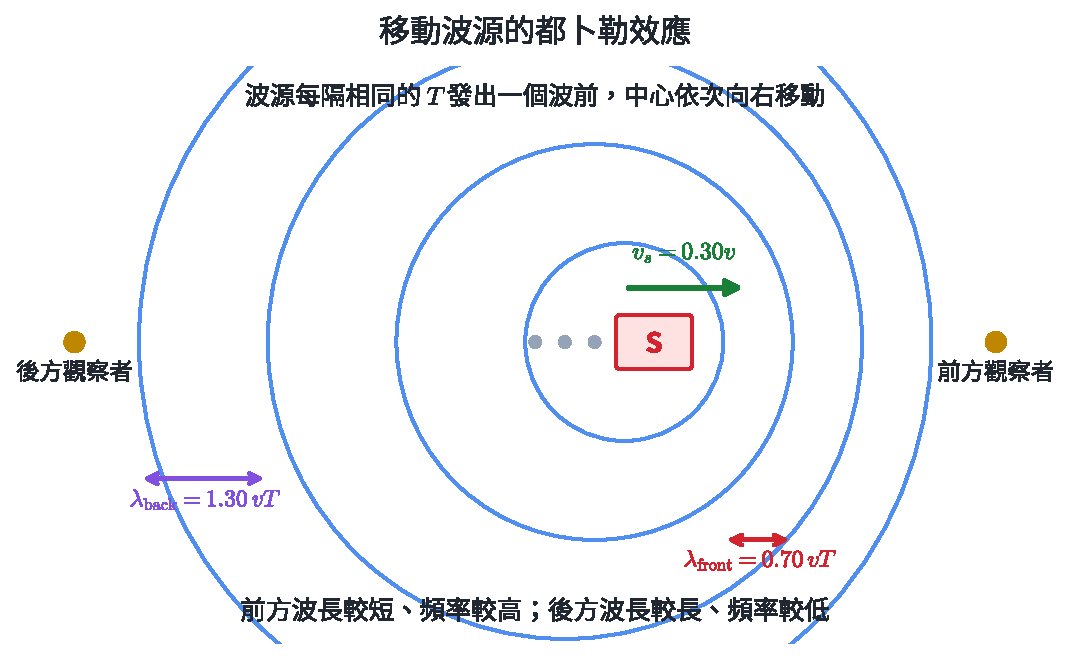
\includegraphics[width=0.94\linewidth,height=\textheight,keepaspectratio,alt={圖 12｜波源向右移動，使前方波長縮短、接收頻率升高；後方波長拉長、接收頻率降低。}]{assets/必物-4-都卜勒波前.pdf}
\caption{圖 12｜波源向右移動，使前方波長縮短、接收頻率升高；後方波長拉長、接收頻率降低。}
\end{figure}

設波在介質中的速率為 \(v\)，靜止波源頻率為 \(f_0\)、週期為 \(T=1/f_0\)，波源以 \(v_s\) 向右移動，且 \(v_s<v\)。一個週期內：

\begin{itemize}
\tightlist
\item
  前一個波峰前進 \(vT\)；
\item
  波源也向前移動 \(v_sT\)。
\end{itemize}

因此前方相鄰波峰距離為

\[
\lambda_{\text{前}}=(v-v_s)T
=\frac{v-v_s}{f_0},
\]

後方則為

\[
\lambda_{\text{後}}=(v+v_s)T
=\frac{v+v_s}{f_0}.
\]

介質中的波速仍為 \(v\)，所以靜止觀察者接收到

\[
f_{\text{前}}=\frac{v}{\lambda_{\text{前}}}
=f_0\frac{v}{v-v_s}>f_0,
\]

\[
f_{\text{後}}=\frac{v}{\lambda_{\text{後}}}
=f_0\frac{v}{v+v_s}<f_0.
\]

移動觀察者的機制不同：波長在介質中已固定，觀察者向波源移動時，每秒迎接更多波峰，接收頻率升高；遠離時降低。聲音的音量主要與強度、距離和功率有關，音調高低主要由頻率決定。

\subsection{7.2 儀器量到的是視線方向的速度}\label{ux5100ux5668ux91cfux5230ux7684ux662fux8996ux7ddaux65b9ux5411ux7684ux901fux5ea6}

都卜勒效應只由波源與觀察者沿兩者連線的相對運動造成。物體速度為 \(u\)，速度方向與視線夾角為 \(\alpha\) 時，徑向分量為

\[
u_r=u\cos\alpha.
\]

物體橫越視野、瞬間與視線垂直時，\(\alpha=90^\circ\)，徑向分量為零；即使物體移動很快，當下的都卜勒頻移也可為零。

應用包括：

\begin{itemize}
\tightlist
\item
  醫學都卜勒超音波：由血球散射回波的頻移估計血流徑向速度。
\item
  雷達測速：由反射電磁波的頻移估計車輛靠近或遠離的速度分量。
\item
  天文光譜：譜線向紅端移表示遠離，向藍端移表示接近；測到的是視線速度。
\item
  氣象雷達：由降水粒子回波的頻移估計風場與降水運動。
\end{itemize}

機械波公式中的 \(v\) 是相對介質的波速；電磁波在真空中的高速運動需使用相對論都卜勒關係。本章日常聲波與低速雷達情境著重頻移方向、波前幾何與徑向分量。

\begin{HandoutWorkedExample}

\subsection{完整示範 20｜救護車通過前後的音調}\label{ux5b8cux6574ux793aux7bc4-20ux6551ux8b77ux8ecaux901aux904eux524dux5f8cux7684ux97f3ux8abf}

救護車鳴笛並朝靜止行人靠近。波源朝行人移動，前方波長縮短，行人接收頻率高於警笛原頻率。救護車通過後開始遠離，行人位於波源後方，波長拉長，接收頻率低於原頻率。

通過附近時音量也常先增後減，因距離先縮短再增加；音調的突然下降對應接收頻率由前方的較高值轉為後方的較低值。兩種聽覺變化有不同物理來源。

\end{HandoutWorkedExample}

\begin{HandoutWorkedExample}

\subsection{完整示範 21｜雷達測得的徑向速度}\label{ux5b8cux6574ux793aux7bc4-21ux96f7ux9054ux6e2cux5f97ux7684ux5f91ux5411ux901fux5ea6}

汽車以 \(25\ \mathrm{m/s}\) 行駛，速度方向與雷達視線夾角為 \(37^\circ\)。雷達頻移對應的徑向速度為

\[
u_r=u\cos37^\circ
\approx(25)(0.80)
=20\ \mathrm{m/s}.
\]

儀器若只以頻移換算速度，得到約 \(20\ \mathrm{m/s}\)。車的實際速率為 \(25\ \mathrm{m/s}\)；視線角度使量測值低於真實速率。雷達對準行車方向時 \(\alpha\) 接近 \(0^\circ\)，徑向速度才接近車速。

\end{HandoutWorkedExample}

\begin{HandoutSelfCheck}

\subsection{本節獨立練習}\label{ux672cux7bc0ux7368ux7acbux7df4ux7fd2-6}

\begin{enumerate}
\def\labelenumi{\arabic{enumi}.}
\tightlist
\item
  靜止觀察者前方有一聲源朝他移動。波速、前方波長與接收頻率，相對聲源靜止時各如何改變？
\item
  聲源靜止，觀察者朝聲源移動。介質中的波長是否改變？接收頻率如何改變？
\item
  一輛車以 \(30\ \mathrm{m/s}\) 行駛，速度方向與雷達視線夾 \(60^\circ\)。徑向速度是多少？
\item
  恆星吸收譜線相對實驗室波長向長波方向移動。恆星沿視線接近或遠離？
\item
  救護車完全靜止但警笛功率提高。遠方觀察者聽到的頻率與強度各如何改變？
\end{enumerate}

\textbf{簡答：}1. 波速不變、前方波長縮短、頻率升高。2. 波長不變，觀察者迎接波峰的速率增加，所以接收頻率升高。3. \(15\ \mathrm{m/s}\)。4. 遠離，稱為紅移。5. 頻率不變，強度增加。

\end{HandoutSelfCheck}

\section{8. 全章分層練習}\label{ux5168ux7ae0ux5206ux5c64ux7df4ux7fd2}

\subsection{A｜核心辨識}\label{aux6838ux5fc3ux8fa8ux8b58}

\subsubsection{第 1 題｜直導線磁場}\label{ux7b2c-1-ux984cux76f4ux5c0eux7ddaux78c1ux5834}

直導線電流穿出紙面。求導線正右方與正上方兩點的磁場方向。

\subsubsection{第 2 題｜圓形線圈}\label{ux7b2c-2-ux984cux5713ux5f62ux7ddaux5708}

圓形線圈由紙面正面看為逆時針電流。

\begin{enumerate}
\def\labelenumi{\arabic{enumi}.}
\tightlist
\item
  線圈中心磁場朝紙面內或外？
\item
  幾何與介質不變，電流加倍時，中心磁場近似如何改變？
\end{enumerate}

\subsubsection{第 3 題｜冷次定律}\label{ux7b2c-3-ux984cux51b7ux6b21ux5b9aux5f8b}

磁鐵 N 極沿線圈軸靠近一閉合線圈，隨後停止。從磁鐵側觀察：

\begin{enumerate}
\def\labelenumi{\arabic{enumi}.}
\tightlist
\item
  靠近時線圈近端的磁極與電流方向為何？
\item
  停止後感應電流如何？
\end{enumerate}

\subsubsection{第 4 題｜週期波}\label{ux7b2c-4-ux984cux9031ux671fux6ce2}

一列波的週期為 \(0.20\ \mathrm s\)，波長為 \(1.5\ \mathrm m\)。求頻率與波速。

\subsubsection{第 5 題｜平面鏡}\label{ux7b2c-5-ux984cux5e73ux9762ux93e1}

光線與平面鏡法線夾 \(50^\circ\) 入射。求反射角，以及入射光線與反射光線的夾角。

\subsubsection{第 6 題｜電磁波譜}\label{ux7b2c-6-ux984cux96fbux78c1ux6ce2ux8b5c}

依波長由長到短排列：紅外線、X 射線、無線電波、紫外線。再指出其中通常具有游離能力的波段。

\subsection{B｜模型運用}\label{bux6a21ux578bux904bux7528}

\subsubsection{第 7 題｜兩平行導線的磁力}\label{ux7b2c-7-ux984cux5169ux5e73ux884cux5c0eux7ddaux7684ux78c1ux529b}

兩條長直導線位於同一平面，彼此平行且電流都向上。畫出左導線在右導線位置的磁場方向，再求右導線所受磁力方向，據此判斷兩線吸引或排斥。

\subsubsection{第 8 題｜線圈進出磁場區}\label{ux7b2c-8-ux984cux7ddaux5708ux9032ux51faux78c1ux5834ux5340}

一矩形閉合線圈向右等速通過有限的均勻磁場區，磁場穿出紙面。分別判斷線圈進入、完全位於磁場內、離開三階段的感應電流方向。

\subsubsection{第 9 題｜變壓器}\label{ux7b2c-9-ux984cux8b8aux58d3ux5668}

理想變壓器初級 \(800\) 匝、次級 \(200\) 匝，初級交流電壓 \(120\ \mathrm V\)。

\begin{enumerate}
\def\labelenumi{\arabic{enumi}.}
\tightlist
\item
  求次級電壓。
\item
  若初級改接穩定 \(120\ \mathrm V\) 直流，穩定後次級電壓為何？
\end{enumerate}

\subsubsection{第 10 題｜家庭支路}\label{ux7b2c-10-ux984cux5bb6ux5eadux652fux8def}

\(110\ \mathrm V\)、額定 \(15\ \mathrm A\) 的支路同時使用 \(660\ \mathrm W\) 電鍋、\(550\ \mathrm W\) 電熱器與 \(770\ \mathrm W\) 吹風機。求總電流並判斷是否過載。

\subsubsection{第 11 題｜折射}\label{ux7b2c-11-ux984cux6298ux5c04}

光由空氣射入折射率 \(\sqrt2\) 的介質，入射角 \(30.0^\circ\)。求折射角，並說明波長如何改變。

\subsubsection{第 12 題｜雙狹縫}\label{ux7b2c-12-ux984cux96d9ux72f9ux7e2b}

波長 \(500\ \mathrm{nm}\) 的單色光照射間距 \(0.25\ \mathrm{mm}\) 的雙狹縫，屏幕距離 \(1.5\ \mathrm m\)。求相鄰亮紋間距。

\subsection{C｜多步推理}\label{cux591aux6b65ux63a8ux7406}

\subsubsection{第 13 題｜反向電流的空間磁場}\label{ux7b2c-13-ux984cux53cdux5411ux96fbux6d41ux7684ux7a7aux9593ux78c1ux5834}

兩條相同長直導線相距 \(2a\)，左導線電流向上、右導線電流向下，量值相同。

\begin{enumerate}
\def\labelenumi{\arabic{enumi}.}
\tightlist
\item
  兩導線中點的磁場同向相加或反向抵消？
\item
  在兩導線外側很靠近左導線的一點，哪一條導線的磁場占優勢？
\item
  兩導線彼此吸引或排斥？
\end{enumerate}

\subsubsection{第 14 題｜磁通量---時間資料}\label{ux7b2c-14-ux984cux78c1ux901aux91cfux6642ux9593ux8cc7ux6599}

單匝線圈的磁通量隨時間變化如下：

{\def\LTcaptype{none} % do not increment counter
\begin{longtable}[]{@{}ll@{}}
\toprule\noalign{}
時間區間 & 磁通量變化 \\
\midrule\noalign{}
\endhead
\bottomrule\noalign{}
\endlastfoot
\(0\) 到 \(2\ \mathrm s\) & 由 \(0\) 線性增至 \(4.0\ \mathrm{mWb}\) \\
\(2\) 到 \(5\ \mathrm s\) & 維持 \(4.0\ \mathrm{mWb}\) \\
\(5\) 到 \(6\ \mathrm s\) & 線性降至 \(0\) \\
\end{longtable}
}

比較三區間感應電動勢的量值與方向。

\subsubsection{第 15 題｜折射資料反推介質}\label{ux7b2c-15-ux984cux6298ux5c04ux8cc7ux6599ux53cdux63a8ux4ecbux8cea}

光由介質 A 進入介質 B，入射角 \(45^\circ\)、折射角 \(30^\circ\)。

\begin{enumerate}
\def\labelenumi{\arabic{enumi}.}
\tightlist
\item
  求 \(v_A/v_B\)。
\item
  求 \(\lambda_A/\lambda_B\)。
\item
  判斷哪一介質折射率較大。
\end{enumerate}

\subsubsection{第 16 題｜移動聲源的前後波長}\label{ux7b2c-16-ux984cux79fbux52d5ux8072ux6e90ux7684ux524dux5f8cux6ce2ux9577}

空氣中聲速為 \(340\ \mathrm{m/s}\)。聲源週期 \(0.010\ \mathrm s\)，以 \(20\ \mathrm{m/s}\) 向右移動。求波源前方與後方相鄰波峰距離。

\section{9. 跨節整合題}\label{ux8de8ux7bc0ux6574ux5408ux984c}

\subsubsection{第 17 題｜手搖發電機、燈泡與能量守恆}\label{ux7b2c-17-ux984cux624bux6416ux767cux96fbux6a5fux71c8ux6ce1ux8207ux80fdux91cfux5b88ux6046}

手搖發電機接上燈泡。學生發現：

\begin{itemize}
\tightlist
\item
  轉得越快，燈泡通常越亮。
\item
  接上燈泡後，比空載時更難轉。
\end{itemize}

用磁通量變化率、感應電流、冷次定律與能量轉換說明兩項觀察。

\subsubsection{第 18 題｜無線充電的幾何與電路}\label{ux7b2c-18-ux984cux7121ux7ddaux5145ux96fbux7684ux5e7eux4f55ux8207ux96fbux8def}

發射線圈以交流電驅動，接收線圈連接整流與充電電路。分別預測並解釋：

\begin{enumerate}
\def\labelenumi{\arabic{enumi}.}
\tightlist
\item
  發射線圈電流振幅增加。
\item
  兩線圈距離增加。
\item
  接收線圈的平面逐漸轉成與發射線圈中心磁場方向平行。
\end{enumerate}

\subsubsection{第 19 題｜雙狹縫資料判讀}\label{ux7b2c-19-ux984cux96d9ux72f9ux7e2bux8cc7ux6599ux5224ux8b80}

三次實驗資料如下：

{\def\LTcaptype{none} % do not increment counter
\begin{longtable}[]{@{}
  >{\raggedright\arraybackslash}p{(\linewidth - 8\tabcolsep) * \real{0.1579}}
  >{\raggedleft\arraybackslash}p{(\linewidth - 8\tabcolsep) * \real{0.2105}}
  >{\raggedleft\arraybackslash}p{(\linewidth - 8\tabcolsep) * \real{0.2105}}
  >{\raggedleft\arraybackslash}p{(\linewidth - 8\tabcolsep) * \real{0.2105}}
  >{\raggedleft\arraybackslash}p{(\linewidth - 8\tabcolsep) * \real{0.2105}}@{}}
\toprule\noalign{}
\begin{minipage}[b]{\linewidth}\raggedright
組別
\end{minipage} & \begin{minipage}[b]{\linewidth}\raggedleft
波長 \(\lambda\)（nm）
\end{minipage} & \begin{minipage}[b]{\linewidth}\raggedleft
狹縫距 \(d\)（mm）
\end{minipage} & \begin{minipage}[b]{\linewidth}\raggedleft
屏距 \(L\)（m）
\end{minipage} & \begin{minipage}[b]{\linewidth}\raggedleft
條紋間距 \(\Delta y\)（mm）
\end{minipage} \\
\midrule\noalign{}
\endhead
\bottomrule\noalign{}
\endlastfoot
A & 600 & 0.20 & 1.0 & 3.0 \\
B & 600 & 0.20 & 2.0 & 6.1 \\
C & 600 & 0.40 & 2.0 & 3.0 \\
\end{longtable}
}

\begin{enumerate}
\def\labelenumi{\arabic{enumi}.}
\tightlist
\item
  A、B 支持哪一個比例關係？
\item
  B、C 支持哪一個比例關係？
\item
  若要用同一裝置比較紅光與藍光波長，哪些量應固定？
\end{enumerate}

\subsubsection{第 20 題｜恆星光譜與速度資訊}\label{ux7b2c-20-ux984cux6046ux661fux5149ux8b5cux8207ux901fux5ea6ux8cc7ux8a0a}

某元素在實驗室的吸收線波長為 \(500.0\ \mathrm{nm}\)，恆星光譜中的同一條線出現在 \(500.8\ \mathrm{nm}\)。

\begin{enumerate}
\def\labelenumi{\arabic{enumi}.}
\tightlist
\item
  這是紅移或藍移？
\item
  恆星沿視線接近或遠離？
\item
  這筆資料能否單獨決定恆星完整的三維速度？說明理由。
\end{enumerate}

\section{10. 全章練習詳解}\label{ux5168ux7ae0ux7df4ux7fd2ux8a73ux89e3}

\subsection{第 1 題詳解}\label{ux7b2c-1-ux984cux8a73ux89e3}

電流穿出紙面時，右手四指沿逆時針繞行。

{\def\LTcaptype{none} % do not increment counter
\begin{longtable}[]{@{}ll@{}}
\toprule\noalign{}
觀察點 & 圓周切線方向 \\
\midrule\noalign{}
\endhead
\bottomrule\noalign{}
\endlastfoot
導線正右方 & 向上 \\
導線正上方 & 向左 \\
\end{longtable}
}

方向圖對應圖 1 左側。磁場與從導線指向觀察點的半徑互相垂直。

\subsection{第 2 題詳解}\label{ux7b2c-2-ux984cux8a73ux89e3}

逆時針電流由右手四指表示，拇指指向紙面外，所以中心磁場穿出紙面。

幾何與介質固定時，\(B\propto I\)。電流加倍，中心磁場近似加倍，方向維持穿出紙面。

\subsection{第 3 題詳解}\label{ux7b2c-3-ux984cux8a73ux89e3}

N 極靠近使穿過線圈的原磁通量增加。線圈近端形成 N 極來抵抗靠近；從磁鐵側看，線圈電流為逆時針。方向圖對應圖 3 的靠近狀態。

磁鐵停止後，位置與磁通量固定：

\[
\frac{\Delta\Phi_B}{\Delta t}=0,
\]

所以感應電動勢與感應電流降為零。

\subsection{第 4 題詳解}\label{ux7b2c-4-ux984cux8a73ux89e3}

\[
f=\frac1T=\frac1{0.20}=5.0\ \mathrm{Hz}.
\]

\[
v=f\lambda=(5.0)(1.5)=7.5\ \mathrm{m/s}.
\]

單位檢查：\(\mathrm{Hz\cdot m}=\mathrm{s^{-1}m}=\mathrm{m/s}\)。

\subsection{第 5 題詳解}\label{ux7b2c-5-ux984cux8a73ux89e3}

題目角度由法線量起，因此

\[
\theta_r=\theta_i=50^\circ.
\]

入射光與反射光分處法線兩側，夾角為

\[
\theta_i+\theta_r=100^\circ.
\]

若題目改給光線與鏡面的夾角，才需要先取餘角。

\subsection{第 6 題詳解}\label{ux7b2c-6-ux984cux8a73ux89e3}

波長由長到短：

\[
\text{無線電波}\rightarrow\text{紅外線}
\rightarrow\text{紫外線}\rightarrow\text{X 射線}.
\]

紫外線與 X 射線的光子能量較高，通常列為具有游離能力的波段；風險仍與強度、時間及吸收量有關。

\subsection{第 7 題詳解}\label{ux7b2c-7-ux984cux8a73ux89e3}

取紙面向右為 \(+x\)、向上為 \(+y\)、穿出紙面為 \(+z\)。參與判斷的方向圖為：

{\def\LTcaptype{none} % do not increment counter
\begin{longtable}[]{@{}
  >{\raggedright\arraybackslash}p{(\linewidth - 4\tabcolsep) * \real{0.3333}}
  >{\raggedright\arraybackslash}p{(\linewidth - 4\tabcolsep) * \real{0.3333}}
  >{\raggedright\arraybackslash}p{(\linewidth - 4\tabcolsep) * \real{0.3333}}@{}}
\toprule\noalign{}
\begin{minipage}[b]{\linewidth}\raggedright
左導線
\end{minipage} & \begin{minipage}[b]{\linewidth}\raggedright
導線間
\end{minipage} & \begin{minipage}[b]{\linewidth}\raggedright
右導線
\end{minipage} \\
\midrule\noalign{}
\endhead
\bottomrule\noalign{}
\endlastfoot
電流 \(\uparrow\)，受力 \(\rightarrow\) & 左導線在右側建立 \(\otimes\) 磁場 & 電流 \(\uparrow\)，受力 \(\leftarrow\) \\
\end{longtable}
}

左導線電流向上。在它右側，右手定則給出磁場穿入紙面，即 \(-z\)。右導線電流為 \(+y\)，因此

\[
\vec F\propto(+y)\times(-z)=-x,
\]

右導線受力向左。由對稱性，左導線受力向右，兩線互相吸引。

\subsection{第 8 題詳解}\label{ux7b2c-8-ux984cux8a73ux89e3}

以穿出紙面磁通量為正，三階段方向表為：

{\def\LTcaptype{none} % do not increment counter
\begin{longtable}[]{@{}llll@{}}
\toprule\noalign{}
階段 & 穿出紙面磁通量 & 感應磁場 & 電流 \\
\midrule\noalign{}
\endhead
\bottomrule\noalign{}
\endlastfoot
進入 & 增加 & 穿入紙面 & 順時針 \\
完全位於均勻場內 & 固定 & 無 & 零 \\
離開 & 減少 & 穿出紙面 & 逆時針 \\
\end{longtable}
}

進入與離開時，線圈和磁場區的重疊面積正在改變；完全進入後雖仍移動，穿過線圈的磁通量固定。

\subsection{第 9 題詳解}\label{ux7b2c-9-ux984cux8a73ux89e3}

理想變壓器：

\[
\frac{V_s}{V_p}=\frac{N_s}{N_p}
=\frac{200}{800}=\frac14.
\]

所以

\[
V_s=\frac14(120)=30\ \mathrm V.
\]

穩定直流使初級磁通量維持固定，穩定後 \(\Delta\Phi_B/\Delta t=0\)，次級感應電壓為零。接通與切斷瞬間可能出現短暫感應。

\subsection{第 10 題詳解}\label{ux7b2c-10-ux984cux8a73ux89e3}

並聯支路中的總功率為

\[
P_{\text{總}}=660+550+770=1980\ \mathrm W.
\]

\[
I_{\text{總}}=\frac{P_{\text{總}}}{V}
=\frac{1980}{110}=18.0\ \mathrm A.
\]

\(18.0\ \mathrm A>15\ \mathrm A\)，支路過載。電流增加會使導線的 \(I^2R\) 發熱快速增加，過電流保護裝置應切斷支路。

\subsection{第 11 題詳解}\label{ux7b2c-11-ux984cux8a73ux89e3}

由司乃耳定律：

\[
(1.00)\sin30.0^\circ
=(\sqrt2)\sin\theta_2.
\]

\[
\sin\theta_2=\frac{1}{2\sqrt2}\approx0.3536,
\qquad
\theta_2\approx20.7^\circ.
\]

介質折射率為 \(\sqrt2\)，光速與波長都變為空氣中近似值的 \(1/\sqrt2\)；頻率由光源決定而保持不變。

\subsection{第 12 題詳解}\label{ux7b2c-12-ux984cux8a73ux89e3}

圖 11 左側給出雙狹縫的幾何關係。先換單位：

\[
\lambda=5.00\times10^{-7}\ \mathrm m,
\qquad
d=2.5\times10^{-4}\ \mathrm m.
\]

\[
\Delta y
=\frac{\lambda L}{d}
=\frac{(5.00\times10^{-7})(1.5)}
{2.5\times10^{-4}}
=3.00\times10^{-3}\ \mathrm m
=3.00\ \mathrm{mm}.
\]

\subsection{第 13 題詳解}\label{ux7b2c-13-ux984cux8a73ux89e3}

兩導線間的任一點，都位於左導線右側、右導線左側。左電流向上在右側建立入紙面磁場；右電流向下在左側也建立入紙面磁場，所以中點兩磁場同向相加。

在兩導線外側且很靠近左導線處，左導線距離較小。由 \(B\propto I/r\)，左導線的磁場占優勢；兩導線貢獻方向相反，合場方向由較近的左導線決定。

對右導線而言，左導線在它的位置建立入紙面磁場；右導線電流向下：

\[
(-y)\times(-z)=+x,
\]

所以右導線受力向右。左導線對稱地向左，兩線互相排斥。

\subsection{第 14 題詳解}\label{ux7b2c-14-ux984cux8a73ux89e3}

感應電動勢量值等於磁通量---時間圖斜率量值：

\[
|\mathcal E|=\left|\frac{\Delta\Phi_B}{\Delta t}\right|.
\]

{\def\LTcaptype{none} % do not increment counter
\begin{longtable}[]{@{}
  >{\raggedright\arraybackslash}p{(\linewidth - 4\tabcolsep) * \real{0.2727}}
  >{\raggedleft\arraybackslash}p{(\linewidth - 4\tabcolsep) * \real{0.3636}}
  >{\raggedleft\arraybackslash}p{(\linewidth - 4\tabcolsep) * \real{0.3636}}@{}}
\toprule\noalign{}
\begin{minipage}[b]{\linewidth}\raggedright
時間區間
\end{minipage} & \begin{minipage}[b]{\linewidth}\raggedleft
斜率
\end{minipage} & \begin{minipage}[b]{\linewidth}\raggedleft
感應電動勢
\end{minipage} \\
\midrule\noalign{}
\endhead
\bottomrule\noalign{}
\endlastfoot
\(0\)--\(2\ \mathrm s\) & \((4.0-0)/2=+2.0\ \mathrm{mWb/s}\) & \(2.0\ \mathrm{mV}\) \\
\(2\)--\(5\ \mathrm s\) & \(0\) & \(0\) \\
\(5\)--\(6\ \mathrm s\) & \((0-4.0)/1=-4.0\ \mathrm{mWb/s}\) & \(4.0\ \mathrm{mV}\) \\
\end{longtable}
}

第三區間量值是第一區間的 2 倍，方向相反；中間區間磁通量固定，因此感應電動勢為零。若線圈有 \(N\) 匝，三個量值都再乘 \(N\)，方向關係不變。

\subsection{第 15 題詳解}\label{ux7b2c-15-ux984cux8a73ux89e3}

由惠更斯折射關係：

\[
\frac{\sin\theta_A}{\sin\theta_B}
=\frac{v_A}{v_B}.
\]

所以

\[
\frac{v_A}{v_B}
=\frac{\sin45^\circ}{\sin30^\circ}
=\sqrt2.
\]

頻率跨邊界保持不變，而 \(\lambda=v/f\)，因此

\[
\frac{\lambda_A}{\lambda_B}
=\frac{v_A}{v_B}
=\sqrt2.
\]

B 中速率較小，所以 \(n_B=c/v_B\) 較大；光由 A 進入 B 時偏向法線。

\subsection{第 16 題詳解}\label{ux7b2c-16-ux984cux8a73ux89e3}

一個週期內，波前前進

\[
vT=(340)(0.010)=3.40\ \mathrm m,
\]

波源前進

\[
v_sT=(20)(0.010)=0.20\ \mathrm m.
\]

參與計算的距離關係為：

{\def\LTcaptype{none} % do not increment counter
\begin{longtable}[]{@{}
  >{\raggedright\arraybackslash}p{(\linewidth - 6\tabcolsep) * \real{0.2000}}
  >{\raggedleft\arraybackslash}p{(\linewidth - 6\tabcolsep) * \real{0.2667}}
  >{\raggedleft\arraybackslash}p{(\linewidth - 6\tabcolsep) * \real{0.2667}}
  >{\raggedleft\arraybackslash}p{(\linewidth - 6\tabcolsep) * \real{0.2667}}@{}}
\toprule\noalign{}
\begin{minipage}[b]{\linewidth}\raggedright
方向
\end{minipage} & \begin{minipage}[b]{\linewidth}\raggedleft
波前距離
\end{minipage} & \begin{minipage}[b]{\linewidth}\raggedleft
波源位移
\end{minipage} & \begin{minipage}[b]{\linewidth}\raggedleft
相鄰波峰距離
\end{minipage} \\
\midrule\noalign{}
\endhead
\bottomrule\noalign{}
\endlastfoot
前方 & \(3.40\ \mathrm m\) & 同向減去 \(0.20\ \mathrm m\) & \(\lambda_{\text{前}}=3.20\ \mathrm m\) \\
後方 & \(3.40\ \mathrm m\) & 反向加上 \(0.20\ \mathrm m\) & \(\lambda_{\text{後}}=3.60\ \mathrm m\) \\
\end{longtable}
}

前方波長較短，後方波長較長，與圖 12 一致。

\subsection{第 17 題詳解}\label{ux7b2c-17-ux984cux8a73ux89e3}

轉速增加時，線圈的磁通量在相同時間內改變更多：

\[
|\mathcal E|\propto\left|\frac{\Delta\Phi_B}{\Delta t}\right|.
\]

感應電動勢增加，使閉合電路中的電流與燈泡功率通常增加，燈泡變亮。

接上燈泡後，感應電流在線圈中建立磁場。依冷次定律，這個磁場造成的轉矩抵抗原來的轉動變化，所以手感更重。手對發電機做的機械功轉成燈泡的光、熱與電路損耗；轉得越快或負載取得的電功率越大，維持轉速所需的機械功率通常也越大。

\subsection{第 18 題詳解}\label{ux7b2c-18-ux984cux8a73ux89e3}

接收線圈的磁通量可寫成

\[
\Phi_B=BA\cos\theta,
\]

其中 \(\theta\) 是磁場與接收線圈面積向量的夾角。

\begin{enumerate}
\def\labelenumi{\arabic{enumi}.}
\tightlist
\item
  發射電流振幅增加，通常使交變磁場振幅增加，接收線圈的磁通量變化率與感應電動勢增加。
\item
  距離增加時，穿過接收線圈的磁場通常減弱，磁通量變化率降低，傳輸功率與效率下降。
\item
  接收線圈平面與磁場方向平行時，面積向量與磁場垂直，\(\theta\approx90^\circ\)，所以 \(\Phi_B\approx0\)。幾何耦合減弱，充電功率下降。
\end{enumerate}

整流與控制電路把接收到的交流電轉成適合電池的直流，並限制電壓、電流與溫度。

\subsection{第 19 題詳解}\label{ux7b2c-19-ux984cux8a73ux89e3}

雙狹縫小角度模型為

\[
\Delta y\approx\frac{\lambda L}{d}.
\]

A 到 B 僅把 \(L\) 由 \(1.0\ \mathrm m\) 加倍到 \(2.0\ \mathrm m\)，\(\Delta y\) 由 \(3.0\) 增至 \(6.1\ \mathrm{mm}\)，在量測誤差內支持 \(\Delta y\propto L\)。

B 到 C 僅把 \(d\) 由 \(0.20\) 加倍到 \(0.40\ \mathrm{mm}\)，\(\Delta y\) 由 \(6.1\) 降至 \(3.0\ \mathrm{mm}\)，支持 \(\Delta y\propto1/d\)。

比較紅、藍光波長時，應固定狹縫距離 \(d\)、屏距 \(L\)、同一級數的量測方式與裝置幾何；再由條紋間距比較 \(\lambda\)。同一裝置下，條紋較疏的光波長較長。

\subsection{第 20 題詳解}\label{ux7b2c-20-ux984cux8a73ux89e3}

觀察波長 \(500.8\ \mathrm{nm}\) 大於實驗室波長 \(500.0\ \mathrm{nm}\)，譜線向長波端移動，屬於紅移。這表示恆星沿視線方向遠離觀察者。

都卜勒頻移只提供徑向速度資訊。恆星在天空平面內的橫向速度不直接改變這條譜線的都卜勒位移，因此單一譜線位移無法決定完整三維速度；還需要自行運動、距離等額外資料。

\section{11. 核心整理}\label{ux6838ux5fc3ux6574ux7406}

{\def\LTcaptype{none} % do not increment counter
\begin{longtable}[]{@{}
  >{\raggedright\arraybackslash}p{(\linewidth - 6\tabcolsep) * \real{0.2500}}
  >{\raggedright\arraybackslash}p{(\linewidth - 6\tabcolsep) * \real{0.2500}}
  >{\raggedright\arraybackslash}p{(\linewidth - 6\tabcolsep) * \real{0.2500}}
  >{\raggedright\arraybackslash}p{(\linewidth - 6\tabcolsep) * \real{0.2500}}@{}}
\toprule\noalign{}
\begin{minipage}[b]{\linewidth}\raggedright
模型
\end{minipage} & \begin{minipage}[b]{\linewidth}\raggedright
關係
\end{minipage} & \begin{minipage}[b]{\linewidth}\raggedright
圖像與方向判定
\end{minipage} & \begin{minipage}[b]{\linewidth}\raggedright
直接用途
\end{minipage} \\
\midrule\noalign{}
\endhead
\bottomrule\noalign{}
\endlastfoot
直導線磁場 & \(B\propto I/r\) & 拇指沿電流，四指沿磁場 & 指南針、電流感測 \\
線圈磁場 & \(B\propto NI/R\) & 四指沿電流，拇指沿軸向磁場 & 電磁鐵、繼電器 \\
載流導線受力 & \(F=ILB\sin\theta\) & \(\vec F=I\vec L\times\vec B\) & 馬達、揚聲器 \\
磁通量 & \(\Phi_B=BA\cos\theta\) & 面積向量垂直線圈平面 & 感應幾何 \\
電磁感應 & \(|\mathcal E|=N|\Delta\Phi_B/\Delta t|\) & 感應磁場抵抗磁通量變化 & 發電機、感應爐 \\
變壓器 & \(V_s/V_p\approx N_s/N_p\) & 交流磁通量耦合兩線圈 & 輸配電、充電器 \\
家用支路 & \(I=P/V\)、發熱 \(\propto I^2R\) & 並聯支路、火線保護、接地 & 過載與漏電防護 \\
電磁波 & \(\vec E\perp\vec B\perp\) 傳播方向 & \(\vec E\times\vec B\) 指傳播方向 & 通訊、遙測、成像 \\
週期波 & \(f=1/T\)、\(v=f\lambda\) & 波形傳播與質點振動分開 & 聲、光、水波分析 \\
反射 & \(\theta_r=\theta_i\) & 角度由法線量起 & 鏡面、雷達反射 \\
折射 & \(n_1\sin\theta_1=n_2\sin\theta_2\) & 慢介質中偏向法線 & 鏡片、光纖、成像 \\
惠更斯原理 & 次波包絡形成新波前 & 光線垂直波前 & 推導反射與折射 \\
雙狹縫 & \(\Delta r=m\lambda\) 或 \((m+\tfrac12)\lambda\) & 先比較兩路徑長 & 測波長、薄膜與感測 \\
條紋間距 & \(\Delta y\approx\lambda L/d\) & 長波、遠屏、近狹縫使條紋疏 & 精密量測 \\
繞射 & 展開角尺度 \(\sim\lambda/a\) & 孔徑與波長同量級時顯著 & 解析度、聲波繞障 \\
都卜勒效應 & 前方 \(\lambda=(v-v_s)T\)；\(u_r=u\cos\alpha\) & 前方波前密、後方波前疏 & 超音波、雷達、天文 \\
\end{longtable}
}

涉及方向的題目，先畫電流、磁場、法線、波前或運動方向，再把量值關係放入圖中。涉及跨介質的題目，頻率由波源維持；波速與波長隨介質同步改變。涉及量測的題目，結果對應模型中的可觀察量，例如條紋間距對應波長、頻移對應徑向速度。


\end{document}
